\documentclass[a4paper,12 pt]{report}
\usepackage{latexsym}
\usepackage[utf8]{inputenc}



%\usepackage[english]{babel}
\usepackage[italian]{babel}

\usepackage[protrusion=true,expansion=true]{microtype}	
\usepackage{amsmath,amsfonts,amsthm} % Math packages
\usepackage[pdftex]{graphicx}	
\usepackage{mathtools}

\usepackage{hyperref}
\usepackage[table,xcdraw]{xcolor}
\usepackage{setspace}
\usepackage{amssymb}
\usepackage{listings}
\usepackage{url}

\usepackage{xcolor}
\usepackage[T1]{fontenc}
\newcommand\myworries[1]{\textcolor{red}{#1}}

\usepackage{enumitem}
\usepackage{float}
\usepackage{hyperref}
\usepackage{tikz}
\usepackage{multirow}
% \usepackage{todonotes}
\usepackage{placeins}

\usepackage{graphicx}  
\usepackage{array}
\usepackage{booktabs} 
\usepackage{pifont}
\newcommand{\xmark}{\ding{55}}
\newcommand{\cmark}{\ding{51}} 

\usepackage[square,numbers]{natbib}

%per pseudocodice
\usepackage{algorithm} 
\usepackage{algorithmic}
\floatname{algorithm}{Algoritmo}
\renewcommand{\thealgorithm}{\unskip}
\newlength\myindent
\setlength\myindent{2em}
\newcommand\bindent{%
	\begingroup
	\setlength{\itemindent}{\myindent}
	\addtolength{\algorithmicindent}{\myindent}
}
\newcommand\eindent{\endgroup}
\usepackage{listings}
% package italiano
%
% Opzionale
%
%\renewcommand{\contentsname}{Sommario}
%\renewcommand{\listfigurename}{List of Figures}
%\renewcommand{\listtablename}{List of Tables}
%\renewcommand{\bibname}{Bibliografia}
%\renewcommand{\indexname}{Indice}
%\renewcommand{\figurename}{Figura}
%\renewcommand{\tablename}{Tavola}
%\renewcommand{\partname}{Parte}
%\renewcommand{\chaptername}{Capitolo}
%\renewcommand{\appendixname}{Appendice}
%\renewcommand{\abstractname}{Abstract}
% \renewcommand{\footnotesize}{\scriptsize}
%\renewcommand{\today}{\ifcase\month\or
%  Gennaio\or Febbraio\or Marzo\or Aprile\or Maggio\or Giugno\or
%  Luglio\or Agosto\or Settembre\or Ottobre\or Novembre\or Dicembre\fi
%  \space\number\day, \number\year}

% package formato
\pagestyle{plain}
\setlength{\topmargin}{0.0in}
\setlength{\headheight}{0.1in}
\setlength{\headsep}{0.0in}
\setlength{\footskip}{0.8in}
\setlength{\textheight}{9.0in}
\setlength{\textwidth}{6.0in}
\setlength{\oddsidemargin}{0.2in}
\setlength{\evensidemargin}{0.2in}
\setlength{\parindent}{0.4 in}
\onehalfspacing


\def\cent{\centerline}
\def\vs{\vskip 10 pt plus 1 pt}
\def\bs{\bf}
\def\grad{\vec{\nabla}}
\def\gradx{\vec{\nabla}_x}
\def\epsilon{\varepsilon}



\newcommand{\cvd}{\begin{flushright}$\Box$\end{flushright}}
\newcommand{\tr}{{\rm Tr}\;}
\newcommand{\eq}{\begin{equation}}
\newcommand{\feq}{\end{equation}}
\theoremstyle{definition}
\newtheorem{definition}{Definition}[section]
 
\theoremstyle{remark}
\newtheorem*{remark}{Remark}

\definecolor{blu_dmi}{HTML}{002e62}


%%%%%%%%%%%%%%%%%%%%%%%%%%%%%%%%%
%%%%%%%%%%%%%%%%%%%%%%%%%%%%%%%%%
%%%%%%%%%%%%%%%%%%%%%%%%%%%%%%%%%
%%%%%%%%%%%%%%%%%%%%%%%%%%%%%%%%%



\begin{document}

    % Thesis frontmatter --------------------------------------------

\thispagestyle{empty} %suppress page number
\newcommand\hr{\par\vspace{-.5\ht\strutbox}\noindent\hrulefill\par}

\noindent % just to prevent indentation narrowing the line width for this line
\begin{figure}
    \centering
    
\includegraphics[scale=0.8]{Bistarelli/img/Fronte.jpg}
\end{figure}
\centering
\vspace{2cm}
\subsection*{Cybersecurity}
\vspace{2cm}
\Large{Appunti Bistarelli}
\vspace{2cm}
\rule{\textwidth}{0.4pt}
\vspace{2cm}
\small{Anno accademico 2022/2023}

% ------------------------------------------------------------------
    
    \tableofcontents

    \chapter{Costraint Satisfaction Problems} \label{ch:Costraint Satisfaction Problems}
\section{Costraint Satisfaction Problems}
Un vincolo è semplicemente una relazione logica tra diverse incognite (o variabili), ognuna delle quali assume un valore in un dato dominio. Un vincolo quindi restringe i possibili valori che le variabili possono assumere e ne rappresenta alcune informazioni parziali sulle variabili di interesse. 
\vspace{0.5cm}
\\Un CSP o \textbf{Problema di Soddisfacimento di Vincoli} formalmente è una tripla:
\begin{center}
    $(X, D, C)$
\end{center}
\begin{itemize}
    \item X è un insieme finito di \textbf{variabili} $\{x_1, ..., x_n\}$
    \item D è una funzione che associa ad ogni variabile un insieme di valori chiamato dominio, cioè tutti i valori che una variabile può assumere.
    \item C è un \textbf{insieme di vincoli}  $\{c_1, ..., c_n\}$ che delimitano le combinazioni di valori ammissibili per la soluzione del problema. 
    \\Possono essere descritti in maniera:
    \begin{itemize}
        \item $Intenzionale:$ Specifico tutte le tuple che sono permesse (WA $\neq$ NT)
        \item $Estenzionale:$ Utilizzando altre funzioni o predicati, tipo $X_1 = 2X_2$ oppure (WA, NT) $\in$ $\{(red, green), ...\}$.
    \end{itemize}
\end{itemize}
\noindent Alcuni CSP richiedono anche una soluzione che massimizzi una \textbf{funzione obiettivo}. Ciascun vincolo limita la combinazione di valori che un insieme di variabili può assumere contemporaneamente. \\
Per comprendere meglio un problema di soddisfacimento di vincoli è opportuno evidenziare i concetti di stato e di assegnamento:
\begin{itemize}
    \item \textbf{Stato:} Rappresenta ogni combinazione di valori assunti dalle variabili $\{x1,..., xn\}$.
    \item \textbf{Assegnamento:} Rappresenta la soluzione del problema, cioè assegnare dei valori a tutte le variabili (assegnamento completo) in modo tale da soddisfare tutti i vincoli del problema (”assegnamento consistente”). Il compito è trovare una soluzione o tutte le soluzioni. Pertanto, il CSP è un problema combinatorio che può essere risolto mediante la ricerca.
\end{itemize}
\begin{enumerate}
    \item Un assegnamento è \textbf{inconsistente} se viola un vincolo.
    \item Un CSP è \textbf{soddisfacibile} se esiste almeno una soluzione.
    \item Un assegnamento a un sottoinsieme S delle variabili è localmente consistente se soddisfa i vincoli esistenti tra le variabili in S.
\end{enumerate}

\subsection{Constraint Solving}
La risoluzione dei vincoli differisce dalla soddisfazione dei vincoli poiché utilizza variabili con domini infiniti come i numeri reali. Inoltre, i singoli vincoli sono più complicati, ad esempio non lineari, uguaglianze...
\subsection{Esempi}
\subsubsection{Esempio 1}
\textbf{Problema:} Assegnazione delle ore di lezione dei professori (Time Tabling).

\vspace{0.2cm}

\noindent \textbf{Dato}: ”Il prof A non può fare lezione dalle 11 alle 13”, ” Il prof B non può fare lezione nell’Aula B” che sarebbero i vincoli, l’obiettivo è avere un assegnamento per tutte le variabili del problema (che saranno i professori e le aule).
\vspace{0.2cm}

\noindent Il CSP quindi è un modo di rappresentare i problemi attraverso una serie di relazioni.
\vspace{0.2cm}

\subsubsection{Esempio 2}
Lavoriamo in una mappa dell’Australia che mostra ciascuno dei suoi stati e territori e il compito ci viene affidato è di colorare ogni regione di rosso, verde o blu in modo tale che le regioni vicine non hanno lo stesso colore. Per formulare questo come un CSP, definiamo le variabili come le regioni: WA, NT, Q, NSW , V , SA e T. Il dominio di ciascuna variabile è l’insieme $\{rosso, verde, blu\}$. I vincoli richiedono che le regioni vicine abbiano colori distinti; ad esempio, le combinazioni consentite per WA e NT sono le coppie
\begin{center}
    $\{(rosso, verde), (rosso, blu), (verde, rosso), (verde, blu), (blu, rosso), (blu, verde)\}$ 
\end{center}
Ci sono molte soluzioni possibili, come \{W A = rosso, AN D = verde, A = rosso, N SW = verde, V = rosso, SA = blu, T = rosso\}. 
\\È utile visualizzare un CSP come grafico di vincoli. I nodi del grafico corrispondono a variabili del problema e gli archi corrispondono a vincoli
\begin{figure}[htp]
	\centering
    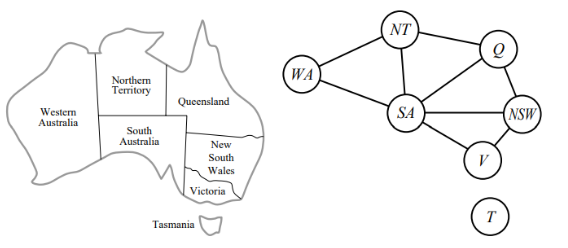
\includegraphics[width=10cm, keepaspectratio]{img/Cap1/map-coloring1.png}
    \caption{Map-Colouring}
\end{figure}
\begin{figure}[htp]
	\centering
    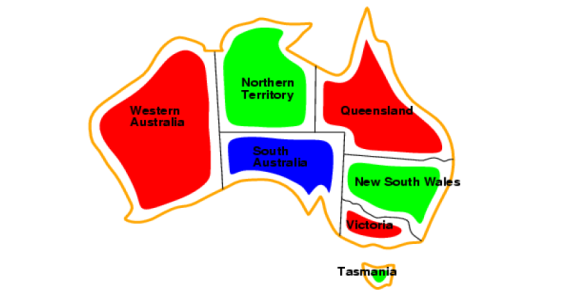
\includegraphics[width=10cm, keepaspectratio]{img/Cap1/map-coloring2.png}
    \caption{Soluzione Map-Colouring}
\end{figure}

\noindent In un CSP binario ogni vincolo è in relazione con due variabili. Il tipo più semplice di CSP coinvolge variabili che sono discrete e hanno domini finiti, i problemi di colorazione della mappa sono di questo tipo.

\subsection{Tipi di CSP}
I CSP si suddividono in base ai tipi delle variabili e dei vincoli:
\subsection{Tipi di Variabili}
Le variabili \textbf{discrete} possono avere domini:
\begin{itemize}
    \item \textbf{Finiti:} grandezza dell’assegnamento completo $d \rightarrow O(d^n)$;
    \item \textbf{Infinti:} 
    \begin{itemize}
        \item hanno bisogno di un linguaggio di vincoli
        \item i vincoli lineari sono risolvibili, i non lineari sono indecidibili;
    \end{itemize}
\end{itemize}
Le variabili \textbf{continue}:
\begin{itemize}
    \item Tempo di inizio e fine per specifici problemi (Hubble telescope)
\end{itemize}
Le variabili continue con dei vincoli lineari sono risolvibili in un tempo polinomiale
dai metodi LP.

\subsection{Tipi di vincoli}
\begin{itemize}
    \item \textbf{Unari:} I vincoli coinvolgono una singola variabile. $SA \neq green$
    \item \textbf{Binari:} I vincoli coinvolgono coppie di variabili. SA $\neq$ W A
    \item \textbf{High order:} I vincoli coinvolgono tre o più variabili.
    \item \textbf{Preferences:} Ho una preferenza su un valore piuttosto che un altro per una certa variabile. Questi sono anche chiamati vincoli Soft, che rappresentano un costo per ogni $assegnamento$ di variabile.
\end{itemize}
Inoltre i vincoli possono essere espressi in maniera:
\begin{itemize}
    \item \textbf{Implicita:} non viene direttamente indicata la relazione fra gli elementi del dominio che sono permessi. Un esempio può essere x<y, dove non si elencano tutti i possibili assegnamenti delle variabili che non violano quel vincolo ma si possono calcolare;
    \item \textbf{Esplicita:} si elencano tutti i valori ammessi per le variabili coinvolte nel vincolo. 
\end{itemize}
Nell’esempio precedente si avranno tutte le coppie di valori ammessi in base a quel
vincolo.

\subsection{Caratteristiche e Proprietà CSP}
\begin{enumerate}
    \item \textbf{Commutatività:} Si considera l’assegnamento di una singola variabile per volta.
    \item \textbf{Monotonicità:} Appena un vincolo viene violato posso interrompere la ricerca perchè sono sicuro che non esisterà soluzione.
    \item \textbf{L’ordine} con il quale seleziono le variabili e assegno i valori è molto importante, abbiamo bisogno di euristiche intelligenti.
    \item \textbf{Indipendenza:} quando le variabili non hanno vincoli tra di loro (come ad esempio sulla mappa dell’Australia c’era la T che non era collegata agli altri nodi), il problema si può decomporre in sotto problemi che possono essere risolti in modo indipendente.
    \item É applicabile un controllo per \textbf{consistenza:} Invece di fare un controllo di consistenza alla fine, lo faccio ad ogni passo.
    \item Possono essere un caso speciale di un problema di ricerca.
\end{enumerate}
\subsection{Standard search formulation}
Gli stati sono definiti dal valore assegnato finora:
\begin{itemize}
    \item \textbf{Stato iniziale: }assegnamento vuoto \{\};
    \item \textbf{Funzione successore: }assegna un valore a una variabile non assegnata che non va in conflitto con l’assegnamento corrente;
    \item \textbf{Goal test: }l’assegnamento corrente è completo. Questa formula viene usata per tutti i CSP e ogni soluzione appare a profondità n con n variabili. Il cammino è irrilevante, così che può usare la formulazione complete-state.
\end{itemize}


\chapter{Metodi di ricerca sistematici} \label{ch:Metodi di ricerca sistematici}
\section{Metodi di ricerca sistematici}
I CSP sono problemi combinatori, quindi si deve trovare una soluzione su tutte le possibili combinazioni di assegnamenti che si possono avere in maniera tale da soddisfare tutti i vincoli. I vari metodi per fare questo sono:
\begin{enumerate}
    \item \textbf{Generate and Test: }Probabilmente il metodo di risoluzione dei problemi più generale. L’algoritmo consiste nei seguenti due passaggi che si ripetono:
    \begin{enumerate}
        \item si generano le etichette
        \item si controlla se vanno bene gli assegnamenti.
    \end{enumerate}
    Alcuni possibili miglioramenti sono ad esempio uno smart generator, ovvero si assegnano i valori alle variabili e se non vanno bene si effettuano dei cambiamenti sugli assegnamenti errati (ricerca locale). Un altro miglioramento consiste nel fare il test sugli assegnamenti e poi fare backtracking.
    \item \textbf{Check and Instantiate: }Assegno uno alla volta i valori alle variabili verificando di non violare i vincoli presenti.
    \item \textbf{Backtraking:} Assegno uno alla volta i valori alle variabili finchè non violo un vincolo; appena lo violo, torno indietro nell’assegnamento. Si estende quindi una soluzione parziale verso una soluzione completa.
\end{enumerate}


\subsection{Backtraking nel dettaglio}
Supponiamo di avere un problema CSP con 4 variabili (A,B,C,D), supponiamo che i vincoli siano
\begin{center}
    $A = D, B \neq D, A + C < 4$
\end{center}
L’algoritmo consiste in:
\begin{enumerate}
    \item Assegna il valore alla variabile;
    \item Si controlla la consistenza;
    \item Finchè tutte le variabili sono etichettate;
\end{enumerate}
\begin{figure}[htp]
	\centering
    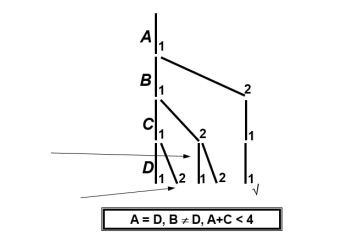
\includegraphics[width=10cm, keepaspectratio]{img/Cap2/back1.png}
    \caption{Esempio backtracking}
\end{figure}
Se tutte le variabili non sono etichettate si torna al passo 1. L’assegnamento delle variabili è commutativo ad esempio
\begin{center}
    $[WA = red$ allora $NT = green]$ come [$NT=green$ allora $WA =red]$
\end{center}


Si devono solo considerare gli assegnamenti alle singole variabili per ogni nodo $\rightarrow$ b = d
e ci sono $d^n$ foglie. 
\\La \textbf{DFS} per i CSP son gli assegnamenti a variabili singole è chiamata ricerca \textbf{backtracking}, essa è l’algoritmo base uniformed per i CSP.
\begin{figure}[htp]
	\centering
    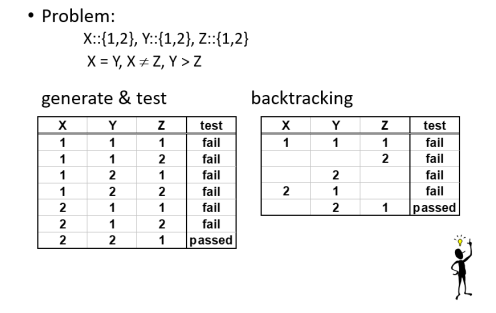
\includegraphics[width=10cm, keepaspectratio]{img/Cap2/back2.png}
    \caption{Esempio generate and test vs backtracking}
\end{figure}

\subsubsection{Ricerca backtracking: incrementale}
La strategia di ricerca è la \textbf{DFS (Depth First Search):}
\begin{enumerate}
    \item scegli una variabile non istanziata, scegli un valore dal suo dominio, controlla se qualche vincolo è violato;
    \item se nessun vincolo viene violato, continua la ricerca in modo ricorsivo;
    \item altrimenti, torna indietro: torna alla decisione precedente e fai un’altra scelta.
\end{enumerate}
In termini di grandezza dell’albero di ricerca il numero di foglie è pari a $d^n$, dove n è il numero di variabili e $d = max|D_i|$.

\begin{figure}[htp]
	\centering
    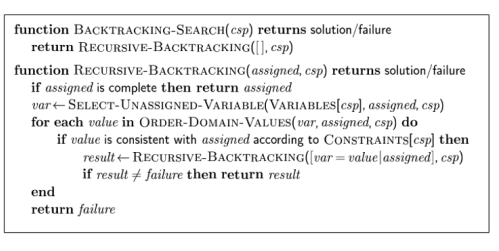
\includegraphics[width=12cm, keepaspectratio]{img/Cap2/dfs.png}
    \caption{Algoritmo di backtracking.}
\end{figure}
\begin{figure}[htp]
	\centering
    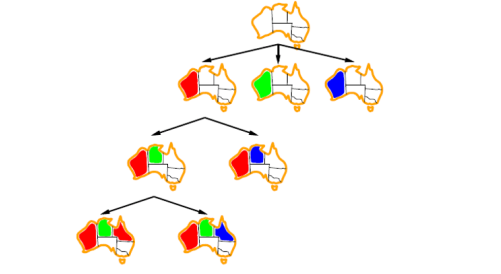
\includegraphics[width=12cm, keepaspectratio]{img/Cap2/dfs2.png}
    \caption{Esempio backtracking.}
\end{figure}
\subsubsection{Miglioramenti dell’efficienza del backtracking}
Per impostazione predefinita, SELECT-UNASSIGNED-VARIABLE seleziona semplicemente la successiva variabile non assegnata nell’ordine dato dalla lista VARIABLES[csp]. 
\\Questo ordinamento di variabili statiche raramente si traduce nella ricerca più efficiente. Ad esempio, dopo le assegnazioni per WA = rosso e NT = verde, c’è un solo valore possibile per SA, quindi ha senso assegnare SA = blue next piuttosto che assegnare Q. Infatti, dopo l’assegnazione di SA, le scelte per Q, NSW e V sono tutte forzate.

\textbf{Variabile più vincolata.} Con questo approccio si va a scegliere, fra le variabili disponibili per l’assegnamento, quella più vincolata in base ad alcune caratteristiche:
\begin{itemize}
    \item si sceglie la variabile con il \textbf{minor numero di valori legali} (minimum remaining values-MRV). È stata anche chiamata la "variabile più vincolata" o euristica "fail-first", quest’ultima perché seleziona una variabile che ha maggiori probabilità di causare un errore presto, potando così l’albero di ricerca.
    \begin{figure}[htp]
    	\centering
        
\includegraphics[width=12cm, keepaspectratio]{img/Cap2/m1.png}
    \end{figure}
    \item si sceglie la variabile con \textbf{più vincoli possibili} (degree heuristic) sulle variabili rimanenti.
    \begin{figure}[htp]
    	\centering
        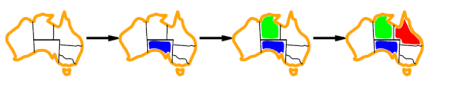
\includegraphics[width=12cm, keepaspectratio]{img/Cap2/m2.png}
    \end{figure}
    \item data una variabile, si sceglie \textbf{il valore meno vincolante} (least-constraining-value), quello che esclude il minor numero di valori nelle restanti variabili.
    \begin{figure}[htp]
    	\centering
        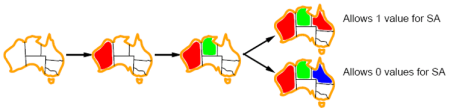
\includegraphics[width=12cm, keepaspectratio]{img/Cap2/m3.png}
    \end{figure}
\end{itemize}

\section{Propagazione delle informazioni attraverso vincoli}
Finora il nostro algoritmo di ricerca considera i vincoli su una variabile solo nel momento in cui il variabile viene scelta da SELECT-UNASSIGNED-VARIABLE. Ma guardando alcuni dei vincoli all’inizio della ricerca, o anche prima dell’inizio della ricerca, possiamo drasticamente ridurre lo spazio di ricerca.
\subsection{Forward Checking}
\textbf{Forward Checking: }  Prima di assegnare una variabile controlla che questo assegnamento mi renda possibile futuri assegnamenti ad altri nodi, poichè se dopo l’assegnamento un dominio per una variabile diventasse vuoto, non si avrebbe soluzione e quindi l’assegnamento non andrebbe nemmeno provato.
\\\textbf{Euristica utilizzata: }  Elimina i valori dal dominio quando viene fatto un
assegnamento ad una variabile, \textbf{se un dominio diventa vuoto, interrompi la ricerca poichè la soluzione non esiste con gli assegnamenti fatti}. Questo metodo offre spesso una soluzione senza avere backtrack.
\begin{figure}[htp]
    \centering
    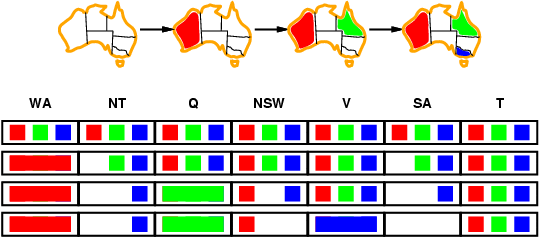
\includegraphics[width=12cm, keepaspectratio]{latex/img/Cap2/forwod1.png}
\end{figure}
\begin{figure}[htp]
    \centering
    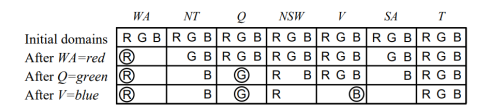
\includegraphics[width=11cm, keepaspectratio]{img/Cap2/f2.png}
    \caption{Forward checking applicata a Map-colouring problem.}
\end{figure}
\\Ci sono due punti importanti da notare su questo esempio. Innanzitutto, si noti che dopo aver assegnato WA = rosso e Q = verde, i domini di NT e SA sono ridotti ad un unico valore; abbiamo eliminato del tutto la ramificazione su queste variabili di propagare le informazioni da WA e Q. L’euristica MRV, che è un partner ovvio per il controllo in avanti, selezionerebbe automaticamente SA e NT successivamente.
\subsection{Constraint propagation}
Sebbene il forward checking rilevi molte incoerenze, non le rileva tutte. Per esempio, consideriamo la terza riga della Figura 1.7. Essa mostra che quando WA è rosso e Q è verde, sia NT che SA sono costretti a essere blu ma questo non è possibile perchè sono due zone vicine. Il forward checking non rileva questo come un’incoerenza, perché non guarda abbastanza avanti. La propagazione del vincolo (constraint propagation) è il termine generale per propagare le implicazioni di un vincolo su una variabile su altre variabili; in questo caso dobbiamo propagare da WA e Q su NT e SA, e quindi sul vincolo tra NT e SA per rilevare l’incoerenza.

\chapter{Local Search per CSP: Consistenza locale - Local Consistency} \label{ch:Local Search per Crisp CSP: Consistenza locale}
\section{Local Consistency}
\textbf{La consistenza locale} è la condizione che si verifica quando ogni nodo di una rete soddisfa tutti i vincoli che lo coinvolgono. Quest’ultima nei CSP consente di \textbf{ridurre lo spazio di ricerca} di un algoritmo eliminando dal dominio delle variabili i valori che non rispettano i vincoli, cioè che non hanno \textbf{supporto}; può essere definita in rapporto alla consistenza di nodo, arco o cammino.
\begin{itemize}
    \item \textbf{Consistenza di Nodo:} Consiste nella verifica dei valori del dominio di un nodo rispetto ai vincoli del nodo stesso. Ad esempio, se il dominio del nodo $x_1$ è pari a 1,2,3 e il vincolo unario di $x_1$ è $x_1 > 1$, la consistenza di nodo consente di ridurre il dominio di x1 a 2,3 riducendo il processo di ricerca dell’algoritmo.
    \item \textbf{Consistenza di Arco:} Consiste nella verifica dei valori di un dominio di un nodo rispetto ai vincoli binari con un altro nodo. Ad esempio, dati due nodi $x_1$ e $x_2$ con rispettivi domini 1,2,3 e 1,4,5,9, il vincolo $x_2 = x_{1}^2$ consente di ridurre il dominio del nodo x2 a 1,4,9 poichè non sussiste alcun nesso tra il valore 5 dell’insieme dominio di $x_2$ e qualsiasi altro elementi dell’insieme dominio di $x_1$.
    \item \textbf{Consistenza di Cammino:} Consiste nella verifica dei valori di un nodo rispetto ai vincoli n-ari con altri n nodi. La consistenza di cammino è un estenzione della consistenza di arco ed è detta anche k-consistenza. Si distingue dalla consistenza di arco che, invece, è dedicata ai vincoli binari tra due nodi.
\end{itemize}

\subsection{Node Consistency}
In questo caso tutti i vincoli sono unari, le variabili sono rappresentate da dei \textbf{vertici}. Il vertice è \textbf{node consistent} se ogni valore nel dominio delle variabili soddisfa tutti i vincoli unari imposti sulla variabile X. Spesso vengono rappresentati come un cappio o arco che ritorna sullo stesso nodo.
\begin{figure}[htp]
	\centering
    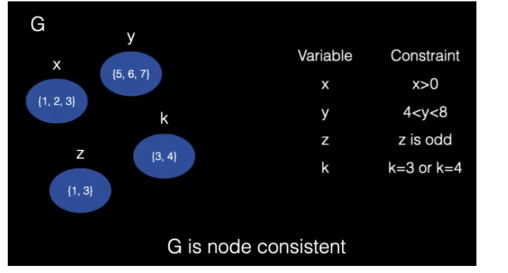
\includegraphics[width=10cm, keepaspectratio]{img/Cap3/node1.png}
    \caption{Esempio grafo node consistent}
\end{figure}

\subsection{Domain Consistency}
L’idea di arc consistency fornisce un metodo veloce di propagazione dei vincoli sostanzialmente più forte del forward checking. Una variabile è consistente al dominio (domain consistent) se nessun valore del dominio del nodo è è dichiarato impossibile da uno qualsiasi dei vincoli. L’idea è di "potare" il più possibile prima di selezionare un valore per le variabili. La domain consistency è stata definita solo per i vincoli che coinvolgono una sola variabile. Quando i vincoli sono binari, possiamo usare gli archi per indicare che un vincolo vale tra una coppia di variabili:
\begin{itemize}
    \item \textbf{un nodo} per ogni variabile
    \item \textbf{un arco} per ogni vincolo
\end{itemize}

\subsection{Arc Consistency}
Quando tutti i vincoli sono binari si parla di arc consistency. Un arco (u,c) è consistente se per ogni valore x del dominio dom(u) esiste un valore y nel dom(v) tale che un assegnamento $u=x$ e $v=y$ soddisfa tutti i vincoli binari che coinvolgono sia u che v.
\subsubsection{Punto fisso e supporto}
Tutto il processo di consistenza locale viene applicato fin quando non si riesce a trovare un punto fisso, cioè fino a quando il dominio delle variabili resta invariato.
\vspace{0.5cm}

 \textbf{Problema arc-consistente:} Un problema nel quale applicando local consistency, nessun dominio di nessuna variabile viene modificato. \\
\noindent \textbf{Supporto:} Per la riduzione dobbiamo vedere quali elementi hanno supporto in Y, ovvero quali hanno un assegnamento in Y tale per cui il vincolo viene soddisfatto.
\begin{figure}[htp]
	\centering
    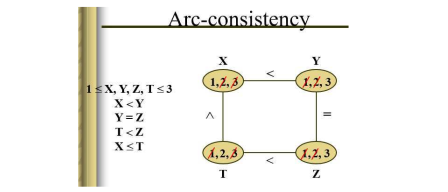
\includegraphics[width=13cm, keepaspectratio]{img/Cap3/esempio-arc.png}
    \caption{Esempio arc-consistency}
\end{figure}
\begin{center}
    Quando $X=1$ esiste un elemento in Y tale per cui $X < Y$? Si, 2,3
    \\Quando $X=2$ esiste un elemento in Y tale per cui $X < Y$? Si, 3
    \\Quando $X=3$ esiste un elemento in Y tale per cui $X < Y$?
    \\No, quindi posso eliminare 3 il dominio di X    
\end{center}
L’operazione che ho fatto si chiama Local Consistency, ma dato che ho utilizzato il vincolo binario si chiama Arc Consistency.

\noindent \textbf{Conclusione:} In questo caso sono stato molto fortunato perchè ho rimasto 1 solo valore possibile per ogni variabile. Quindi la soluzione è unica e sarà:
\begin{center}
    $X = 1, Y = 3, Z = 3, T = 2$
\end{center}
Se fossi stato meno fortunato comunque avrei ridotto gli elementi del dominio e quindi quando sarei andato a fare la ricerca con backtrack comunque lo spazio di ricerca si sarebbe di molto diminuito (avrei controllano meno assegnamenti)
\vspace{0.3cm}

\subsubsection{\textbf{Vantaggio rispetto a fare solo Backtracking senza prima applicare local consistency}}
Se faccio backtrack il dominio degli stati che vado ad esplorare è esponenziale perchè ad X dovrei moltiplicare tutti i possibili valori di Y, a cui dovrei moltiplicare tutti i possibili valori di Z che moltiplico per tutti i valori possibili per T. All’inizio quindi in quel problema si avevano $3^4 = 81$ possibili assegnamenti, mentre se applico prima Local Consistency il problema diventa polinomiale (facile) rispetto al numero di variabili che coinvolgo (in questo caso lo spazio di ricerca mi si riduce ad 1).

\subsection{Algoritmi per Consistenza Locale}
\subsubsection{Procedura Revise}
Per fare diventare un arco (u,v) consistente si cancellano tutti i valori x dal dom(u) che sono incosistenti con tutti i valori in dom(v).
\\Restituisce true se è stata fatta una modifica al dominio di u.
\begin{figure}[htp]
	\centering
    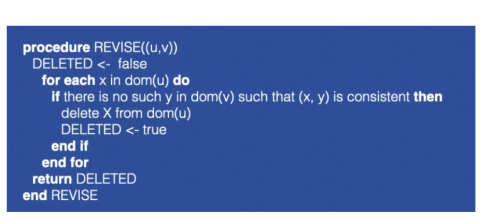
\includegraphics[width=13cm, keepaspectratio]{img/Cap3/revise.png}
    \caption{Procedura REVISE}
\end{figure}

\subsubsection{Algoritmo AC-1}
Un singolo passo dell’agoritmo REVISE non è sufficiente. L’algoritmo base per arc consistecy è AC-1, il quale esegue l’algoritmo REVISE finchè il dominio delle variabili cambia. In questo si ripete la procedura REVISE ogni volta che viene modificato un valore in un dominio.
\begin{figure}[htp]
	\centering
    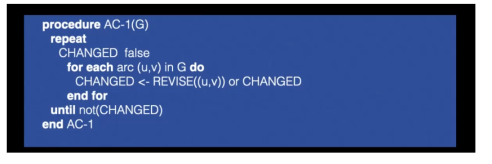
\includegraphics[width=13cm, keepaspectratio]{img/Cap3/ac-1.png}
    \caption{Algoritmo AC-1}
\end{figure}
\\Una sola revisione riuscita di un arco su una particolare iterazione causa la revisione di tutti gli archi nella prossima iterazione anche se gli archi non sono influenzati dal cambiamento.\\
\textbf{L’inefficienza} sta nel fatto che se anche una singola chiamata alla procedura di REVISE su una particolare iterazione risultasse vera, tutti gli archi verrebbero scansionati nuovamente nella successiva iterazione. Questo però non è sempre necessario, perchè la modifica del dominio di una variabile influenza solamente le variabili che sono collegate a X da un vincolo e non le restanti.\\
La complessità temporale è $O(d^3$ * $n$ * $e)$ e quella spaziale è $O(e$ * $n$ * $d)$.

\subsubsection{Algoritmo AC-2}
AC-2 è un algoritmo che può fare arc consistecy in un solo passo attraverso i nodi. Il risultato è ottenuto passando per i nodi in un ordine numerico:
\begin{itemize}
    \item Allegare ad un nodo tutti i valori che non sono in conflitto con i nodi precedentemente assegnati;
    \item Guarda i vicini di questo nodo che sono stati già valutati; se un valore non ha un’assegnazione corrispondente per lo stesso arco, eliminalo;
    \item Ogni volta che qualsiasi valore è cancellato da un arco, guarda ai suoi vicini a sua volta, e controlla se un loro valore può essere eliminato. Se può essere eliminato, si continua il processo iterativamente finchè non ci sono più cambiamenti che possono essere fatti. Poi si prosegue con gli altri archi.
\end{itemize}
In sostanza si sceglie un ordine fra i nodi, prendiamo ad esempio y come primo e controlliamo tutti i vincoli fra y e k se c’è qualche valore di dom(y) che va in conflitto allora si elimina. Stessa cosa si per l’arco (x,y) se si fa qualche modifica si rimette in coda l’arco in modo da controllare se ci sono altre modifiche da fare. Se un valore b del nodo i è rimosso allora si aggiunge tutti (k,i) alla coda Q, per il controllo degli archi.
\begin{figure}[htp]
	\centering
    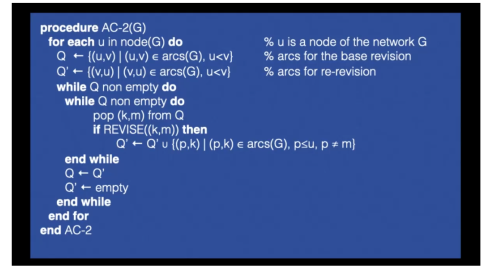
\includegraphics[width=13cm, keepaspectratio]{img/Cap3/ac-2.png}
    \caption{Algoritmo AC-2}
\end{figure}
\\La complessità temporale è $O(d^3$ * $n^2)$ e quella spaziale è $O(n^2$).

\subsubsection{Algoritmo AC-3}
AC-3 è un miglioramento di AC-2, alcuni di essi possono essere già essere nella coda Q. Se è così allora non dovrebbero essere inseriti di nuovo.
\begin{figure}[htp]
	\centering
    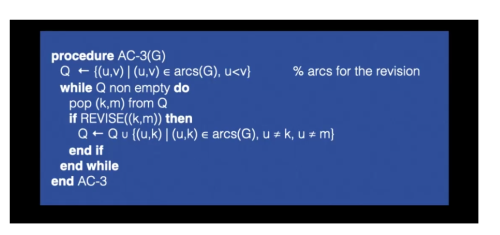
\includegraphics[width=13cm, keepaspectratio]{img/Cap3/ac-3.png}
    \caption{Algoritmo AC-3}
\end{figure}
In sostanza si prende un arco dalla coda Q, si fa la REVISE, se faccio una modifica allora si aggiunge alla coda Q tutti gli archi (u,k) che non sono stati già controllati ovvero $u \neq k$ e $u \neq m$.\\
La complessità temporale è $O(d^2$ * $n^2)$ e quella spaziale è $O(n^2$).

\section{Riassunto del prof}
\subsection{Arc-consistency}
Algoritmo che ha la caratteristica di lavorare a livello locale sul CSP. L’obiettivo è quello di semplificarlo in maniera tale da ridurre la quantità di elementi possibili nel dominio e quindi ridurre il tempo necessario quando faccio la ricerca con backtrack.
\\\textbf{Supporto: } un elemento del dominio di X può essere buttato via se non ha supporto in y.
\begin{figure}[htp]
	\centering
    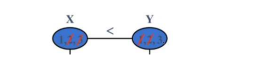
\includegraphics[width=9cm, keepaspectratio]{img/Cap3/riassunto1.png}
\end{figure}
\\Ad esempio, 1 ha supporto in X perchè in Y c’è 2 e 3. Se un elemento non ha supporto lo posso escludere dai valori assegnabili alla variabile. Un problema si dice arc-consistente se ho buttato via tutti gli elementi che NON hanno supporto.

\vspace{0.8cm}

\textbf{Questo è un problema Arc-Consistente?}
\begin{figure}[htp]
	\centering
    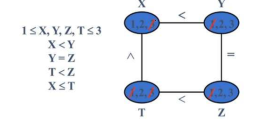
\includegraphics[width=9cm, keepaspectratio]{img/Cap3/riassunto2.png}
\end{figure}
\\No, perchè il 2 andrebbe eliminato da Z. Se riesco a buttare via tutti gli elementi che non hanno supporto allora il problema diventa arc-consistente.

\subsection{Soluzione di un CSP}
La soluzione ad un problema è un assegnamento per tutte le variabili.
\\Nel caso in cui fossi interessato solo ad un sottoinsieme di variabili parliamo di \textbf{Vincolo Distinto.}
Le operazioni sono:
\begin{itemize}
    \item  \textbf{Combinazione} tra i vincoli.
    \item \textbf{Proiezione} nel caso in cui esista questo vincolo distinto.
\end{itemize}
Queste operazioni sono di tipo insiemistico nel caso dei CSP classici (Crisp), nel caso in cui invece passiamo a dei problemi di vincoli Soft, e quindi è presente una nozione di priorità tra le soluzioni (il rosso mi costa più del giallo) parliamo di SCSP.

\subsection{Applicare Local Consistency durante il Backtrack}
L’esempio fatto adesso applica la Local Consistency prima di fare Backtrack. Tuttavia è possibile applicarla anche durante la ricerca con backtrack ogni volta che si modifica il dominio di una variabile, vediamo come: (credo che serva solamente sapere che si può fare anche durante e non l’esempio vero e proprio).
\begin{figure}[htp]
	\centering
    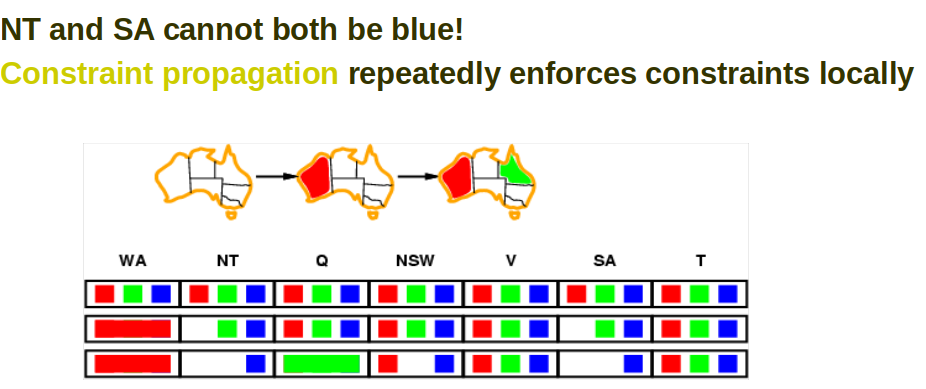
\includegraphics[width=12cm, keepaspectratio]{latex/img/Cap3/prova3.png}
\end{figure}

\subsubsection{L’Arc Consistency è abbastanza per risolvere il problema?}
Se ci dice bene si, come visto sopra (tolgo talmente tante cose che la soluzione me la trova da solo), ma la maggior parte delle volte permette solamente di restringere lo spazio di ricerca, quindi si può rendere un CSP arc-consistente e poi cercare una soluzione con backtracking; oppure assegnare iterativamente un valore e rendere le variabili restanti arco consistenti. Inoltre, se il dominio
di una variabile diventa vuoto, sappiamo che non esisterà soluzione.
\begin{figure}[htp]
	\centering
    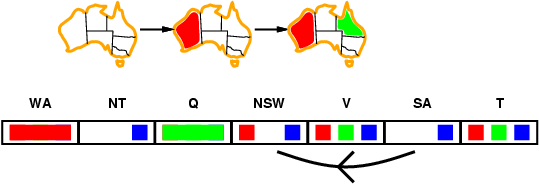
\includegraphics[width=9cm, keepaspectratio]{latex/img/Cap3/prova4.png}
\end{figure}
\begin{figure}[htp]
	\centering
    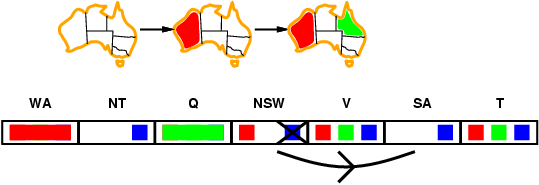
\includegraphics[width=9cm, keepaspectratio]{latex/img/Cap3/prova5.png}
\end{figure}
\begin{figure}[htp]
	\centering
    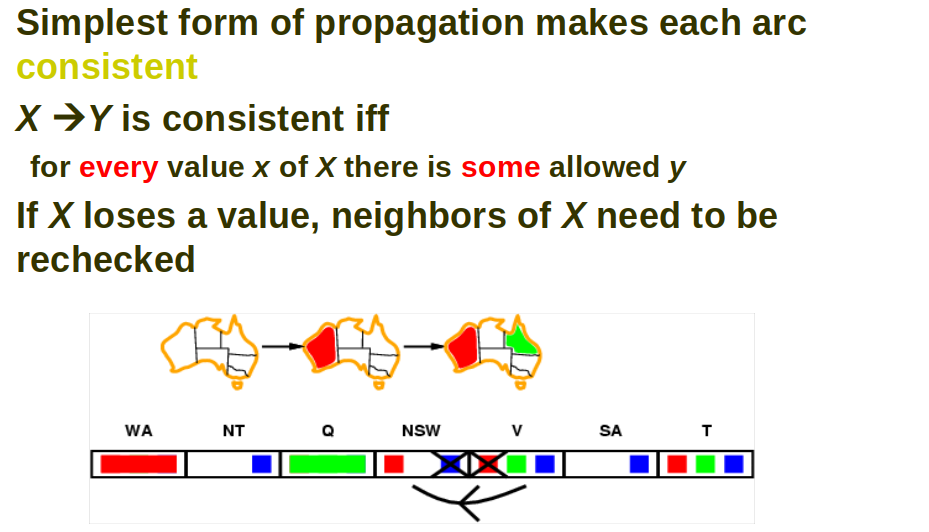
\includegraphics[width=9cm, keepaspectratio]{latex/img/Cap3/prova6.png}
\end{figure}
\begin{figure}[htp]
	\centering
    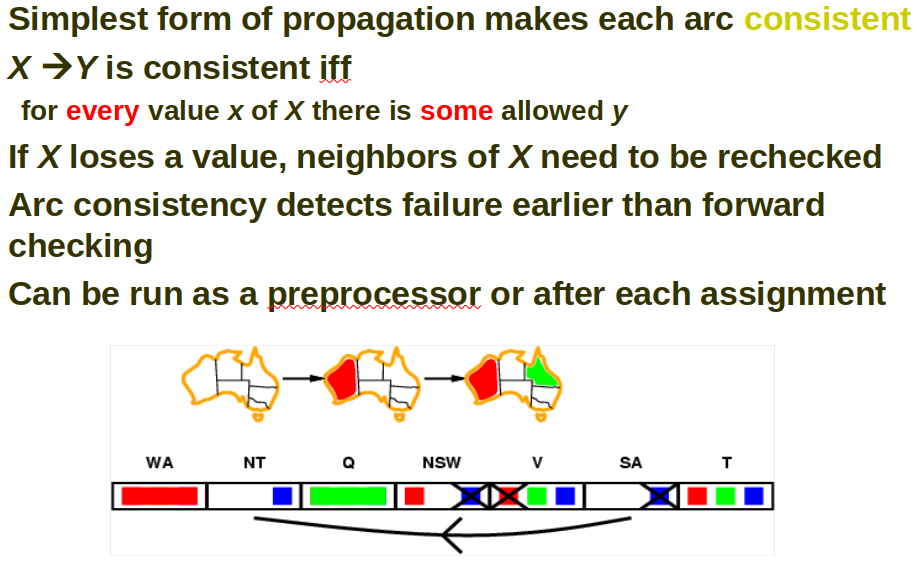
\includegraphics[width=9cm, keepaspectratio]{latex/img/Cap3/prova7.png}
\end{figure}
\subsection{Vincolo distinto (Proiezione)}
Alcune volte non ci interessa sapere il valore che possono ottenere tutte le variabili, ma solamente un sottoinsieme di esse. Definiamo quindi il: 
\\
\textbf{Vincolo distinto (proiezione):} Quali sono gli elementi del problema di cui vogliamo conoscere la soluzione.

\chapter{Soft Constraint Satisfaction Problems} \label{ch:Soft Constraint Satisfaction Problems}
\section{Soft constraint satisfaction Problem (SCSP)}
Un Soft constraint satisfaction Problem (SCSP) è una coppia $<C, con>$ dove:
\begin{itemize}
    \item \textit{C} è un insieme di Vincoli Soft;
    \item \textit{con} è l’insieme delle variabili sulle quali tali vincoli valgono.
\end{itemize}

\subsection{Differenza tra vincoli}
\begin{itemize}
    \item \textbf{Un Vincolo Crisp} delimita l’insieme dei valori ammissibili per una variabile per la soluzione al problema (è quindi una funzione caratteristica che associa ad ogni variabile un assegnamento di 0 o 1 in base a se può assumere o no un certo valore).
    \item \textbf{Un Vincolo Soft} è una funzione che associa ad ogni assegnamento di variabile un valore parzialmente o totalmente ordinato da un insieme di pesi A.
    \\Formalmente è una coppia C $\rightarrow$ $<con, def>$ dove:
    
    \begin{itemize}
        \item \textbf{con} $\subseteq$ V indica per ogni vincolo a quale variabile esso è associato (ad esempio $x_2 $, $x_3$ ).
        \item \textbf{def} è una funzione (è il peso associato ad ogni assegnamento di variabile):
        \begin{center}
            def: $D^k$ $\rightarrow$ A

            Che associa ad ogni elemento del dominio un valore del semiring. 
            \\k rappresenta il numero di variabili.
        \end{center}
    \end{itemize}
\end{itemize}
\textbf{La struttura utilizzata per descrivere problemi di Soft CSP è chiamata semiring.}

\subsection{Esempio}
I vincoli che abbiamo visto in precedenza sono dei vincoli assoluti, la cui violazione esclude una possibile soluzione. Molti dei problemi CSP reali includono i vincoli preference i quali indicano quali soluzioni sono preferite. Per esempio in un problema di timetable in università ci potrebbe essere il professore X che preferisce insegnare la mattina mentre il professore Y preferisce insegnare il pomeriggio. Un timetable dove il prof X insegna alle 14 e il prof Y alle 9 potrebbe essere una soluzione, ma non è quella ottimale viste le preferenze. I vincoli sulle preferenze possono essere codificati spesso come dei costi applicati sugli assegnamenti individuali delle variabili. Riprendendo l’esempio di prima possiamo dare all’assegnamento prof X $=$ (lezione alle 14) un costo di 2, mentre all’assegnamento prof X $=$ (lezione alle 9) un costo di 1. In questo modo si cerca fra le possibili soluzioni quella ottimale andando a minimizzare (o massimizzare...) il costo della soluzione.
\\Supponiamo di avere un problema di colorazione del grafo e cerchiamo di trovare una
soluzione ottimale.
\begin{figure}[htp]
	\centering
    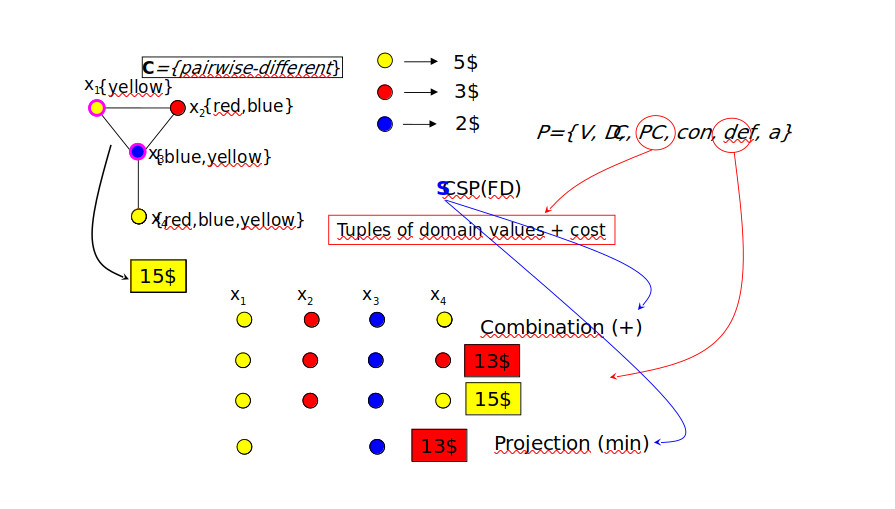
\includegraphics[width=14cm, keepaspectratio]{img/Cap4/scsp2.png}
    \caption{Esempio di SCSP su grafo.}
\end{figure}
\\Partiamo riprendendo la definizione di un CSP, esso è definito come P=\{V,D,C,PC,con,def,a\} i quali indicano:
\begin{itemize}
    \item V $=$ insieme delle variabili;
    \item D $=$ insieme dei domini associati alle variabili;
    \item C $=$ insieme di vincoli, definito come l’associazione variabile-vincolo ovvero quali variabili sono coinvolte in quale vincolo;
    \item PC $=$ sono i vincoli primitivi e variano in base al vincolo e al dominio. A seconda del tipo di vincolo che possiamo avere i primitivi possono essere diversi, esempio se lavoro sugli interi esso conterrà vincoli con gli operatori $<,>,=$.
    \\Sostanzialmente esso indica i tipi di vincoli che posso usare se lavoro su un dominio specifico. Inoltre indicano se il vincolo è implicito (tutti i colori diversi) o esplicito (valgono le coppie $<r,g,b>$, $<g,r,b>$, . . . ).
    \item con $=$ funzione che definisce quali variabili sono coinvolte in quale vincolo, essa dato un vincolo restituisce le variabili che sono connesse a questo;
    \item def $=$ funzione che indica quali sono i valori del dominio possibili per una specifica variabile. In un SCSP questa funzione oltre a dire i valori possibili per una variabile deve indicare anche il costo associato a quei valori, nell’esempio in Figura 4.1 se passiamo in input alla funzione def la variabile x1 essa ci ritornerà come valori possibile il colore giallo con costo 5. Questa è la differenza con la funzione def di un problema CSP.
    \item a $=$ sottoinsieme di V contenente tutte le variabili interessate nella soluzione del SCSP, ad esempio nel caso del grafo abbiamo che le variabili che ci interessano per la soluzione ottimale sono solo $x_1$ e $x_3$ , non tutte quante.
\end{itemize}
Nell’esempio in Figura 4.1 i vincoli binari sono hard, perché la soluzione richiede per forza che i nodi collegati abbiamo colori diversi sennò si violano i vincoli, mentre i vincoli unari (quelli del costo sul colore) sono soft. Nel caso di un CSP quando utilizziamo un algoritmo di ricerca per trovare una soluzione esso si può fermare alla prima soluzione che trova oppure, se richiesto, le cerca tutte quante. Nel caso di SCSP siamo costretti a trovare tutte le possibili soluzioni in modo da scegliere la
migliore. Normalmente si utilizzano due operazioni per trovare la soluzione ottimale in un SCSP:
\begin{itemize}
    \item \textbf{Combinazione (+):} dove metto insieme tutti gli assegnamenti, combinando i vincoli, quindi si calcola anche il costo totale ad esempio con l’operazione di somma;
    \item \textbf{Proiezione (×):} operazione di scelta della soluzione migliore data dalla combinazione in base al minimo o al massimo del costo.
\end{itemize}

\section{Semiring}
Un semiring è una quintupla:
\begin{center}
    $<A, +, x, 0, 1>$
\end{center}
\begin{itemize}
    \item \textbf{A:} l’insieme degli elementi che mi rappresentano i costi (dominio dei costi). Esso può essere l’insieme dei reali oppure un intervallo specifico $[0,1]$
    \item \textbf{+:} operatore di proiezione, usato per fare la scelta fra le soluzioni trovate dalla combinazione, può essere il minimo o massimo. Possiamo definire alcune proprietà:
    \begin{itemize}
        \item \textbf{idempotente:} se faccio a+a dove +=minimo il risultato è sempre a, quando un operatore è idempotente è possibile definire un ordinamento ovvero
        \begin{center}
            $a <= b$ dove b è meglio di a $\Leftarrow \Rightarrow$ $a + b = b$
        \end{center}
    \end{itemize}
    \item \textbf{x:} operatore di combinazione, utilizzato per combinare i vincoli, può essere somma,moltiplicazione etc... dipende dal problema. Possiamo definire alcune proprietà:
    \begin{itemize}
        \item \textbf{commutativa:} si considera il set di vincoli invece delle tuple.
    \end{itemize}
    \item \textbf{0:} rappresenta il valore minimo (peggiore) dell’insieme A, ovvero il bottom sotto il quale non si può andare, per l’intervallo $[0,1]$ è 0;
    \item \textbf{1:} rappresenta il valore massimo (migliore) di A, il top, per l’intervallo $[0,1]$ è 1.
\end{itemize}
Tutti questi che abbiamo visto sono simboli quindi quando si utilizza l’operatore $+$ non si ci si riferisce alla somma ma a un operatore per la proiezione che potrebbe essere minimo o massimo o or.
\subsection{Tipi di Semiring}
\begin{itemize}
    \item \textbf{Probabilistico:} $< R^+ , min, +, +\infty, 0>$ si massimizza la probabilità
    \item \textbf{Weighted:} $<[0, 1] max,x,0,1>$ massimo il costo dato dalla combinazione, dove si fa il prodotto;
    \item \textbf{Fuzzy:} $<[0,1],max,min,0,1>;$
    \item \textbf{Classical:} $<{false,true},$ $\lor$ (OR), $\land$(AND)$, false, true>$
\end{itemize}

\subsection{Esempi pratici SCSP: Domanda esame}
Il vincolo in mezzo è binario, se è $< a, a >$ significa "quando X$=$a e Y$=$a" (perchè è tra le variabili x ed y).
\subsubsection{Esempio con probabilistic}
\begin{figure}[htp]
	\centering
    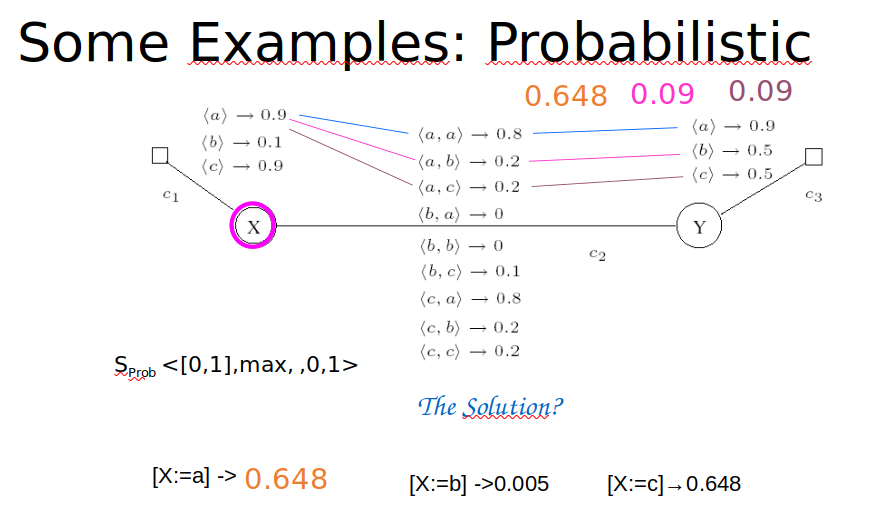
\includegraphics[width=14cm, keepaspectratio]{img/Cap4/probabilistic2.png}
\end{figure}
\noindent \textbf{Descrizione del semiring:} I valori possibili sono tra 0 ed 1, l’operazione
di proiezione è il Massimo; quella di combinazione è la \textbf{moltiplicazione}; il minimo valore è 0; il massimo valore è 1. 
\\Ci domandiamo: Quanto vale l’assegnamento X $=$ a?
\begin{enumerate}
    \item Dato che l’operazione x di combinazione è la moltiplicazione faccio:
    \begin{enumerate}
        \item 0.9*0.8*0.9 = 0.648
        \item 0.9*0.2*0.5 = 0.09
        \item 0.9*0.2*0.5 = 0.09
    \end{enumerate}
    Per poter inserire 0.648 in x = a dovrei dividere per 0.8 i 3 valori su c2 e 0.9 i tre valori su c3 (secondo me).
    \item Dato che l’operazione + di proiezione in questo caso è Max prendo il massimo di tutti gli elementi trovati e quella sarà la soluzione di quando ad X assegno a.
    Facendo lo stesso ragionamento si calcolano tutte le restanti soluzioni.
\end{enumerate}

\subsubsection{Esempio con Fuzzy}
\begin{figure}[htp]
	\centering
    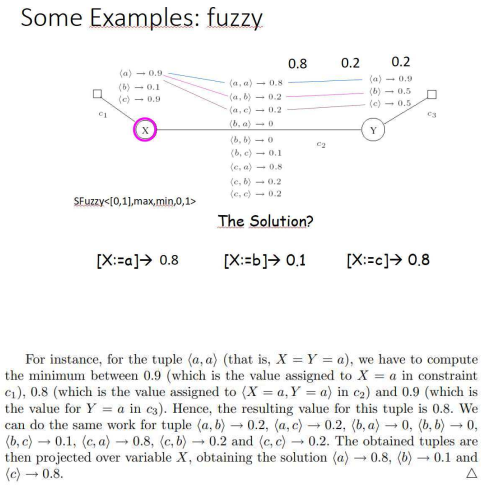
\includegraphics[width=14cm, keepaspectratio]{img/Cap4/fuzzy.png}
\end{figure}

\newpage
\subsubsection{L’aggiunta di vincoli è monotona: peggiora la soluzione}
Questo significa che più aggiungo vincoli e più la soluzione peggiora, più tolgo vincoli più la soluzione mi migliora. Questo perchè più vincoliamo il problema e meno possibilità abbiamo, meno lo vincoliamo e più sono le possibilità. Questo accade nel caso dei vincoli Crisp, nel caso dei vincoli con peso otterremo \textbf{migliori o peggiori} soluzioni.
\subsubsection{Esempio di aggiunta e quindi peggioro}
\begin{figure}[htp]
	\centering
    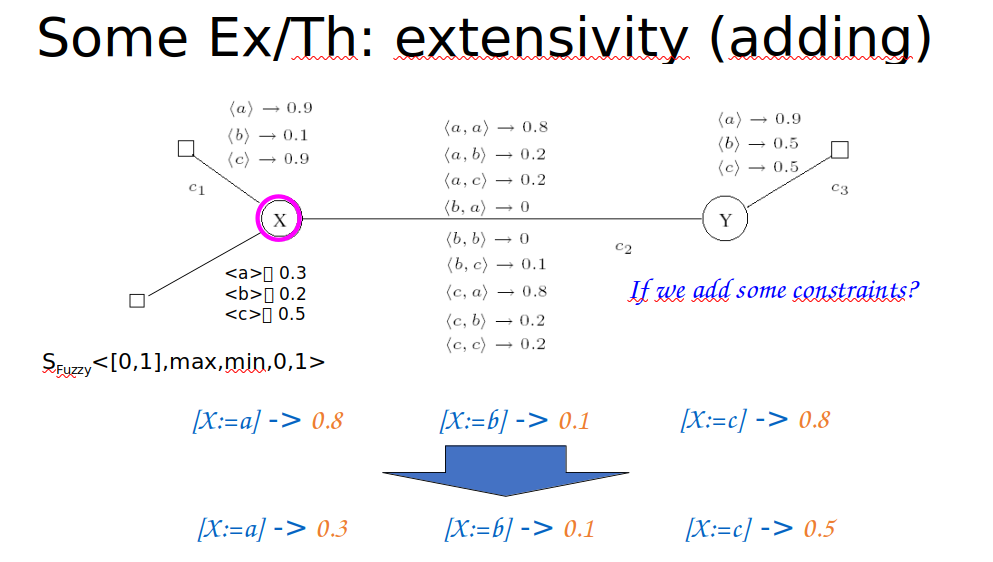
\includegraphics[width=12.5cm, keepaspectratio]{img/Cap4/worst2.png}
\end{figure}

\subsubsection{Esempio di rimozione e quindi miglioro}
\begin{figure}[htp]
	\centering
    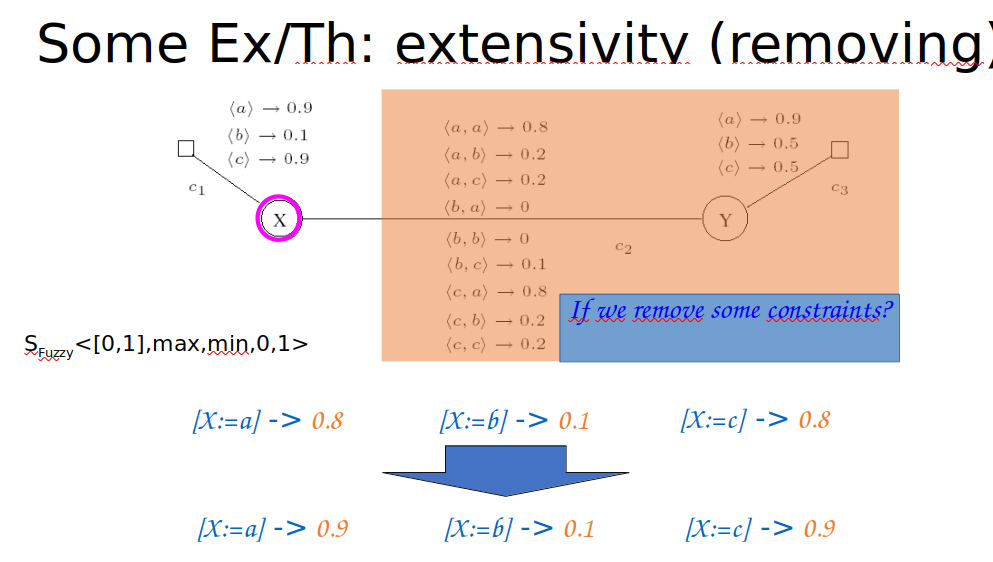
\includegraphics[width=12.5cm, keepaspectratio]{img/Cap4/better2.png}
\end{figure}


\chapter{Local Consistency nei Soft CSP} \label{ch:Local Consistency nei Soft CSP}
\section{Local consistency}
Fare Local consistency nel caso di CSP Soft non significa eliminare dei valori dal dominio, ma significa ridurre (ottimizzare) il valore del semiring associato a quella variabile in maniera tale da fare in modo che questo valore si avvicini il più possibile a quello della soluzione finale.
\subsubsection{Esempio con CSP Soft:}
\begin{figure}[htp]
	\centering
    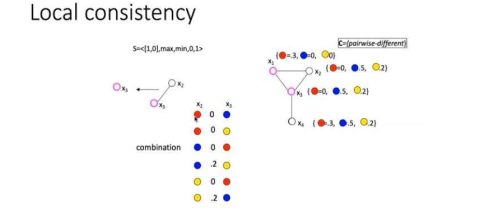
\includegraphics[width=14cm, keepaspectratio]{img/Cap5/LocalConsistency.png}
    % PROBLEMA FOTO
\end{figure}
\noindent In questo esempio sono presenti solo vincoli unari, che mi dice che quando ad $x_1$ gli assegno rosso ha valore 0.3, quando blu o giallo ha valore 0; cosi per tutte le variabili. Siccome il valore 0 è il bottom del semiring, dare 0 significa che non sono assegnamenti permessi, quindi li possiamo direttamente eliminare.\\
\textbf{Ottimizzazione della soluzione su CSP Soft: } Voglio ridurre (ottimizzare) il dominio della variabile $x_3$ , vediamo come fare con tutti i passaggi:
\begin{enumerate}
    \item \textbf{Combinazione:} Prendo tutte le possibili tuple, gli assegno un valore e poi in base all'operatore di combinazione (che in questo caso è min) faccio la proiezione.
    \\Quindi parto cosi:
    Il minimo se $x_2$ è rosso e $x_3$ è blu è 0, perchè è il minimo tra 0 e 0.5.
    \\Il minimo se $x_2$ è rosso e $x_3$ è giallo è 0, perchè è il minimo tra 0 e 0.2.
    \\Continuo cosi per tutte le tuple.
    \\Non ho considerato le coppie di colore uguale perchè c'era scritto $pairwise-different$.
    \item \textbf{Proiezione:} Tra tutti i risultati che genera la combinazione faccio la proiezione sulla variabile in questione, in questo caso $x_3$. Adesso: quanto valore ha $x_3$ quando ha valore rosso? Devo fare il massimo tra 0 e 0 che è 0 e tutto rimane invariato perché $x_3$ sul rosso ha comunque 0. Per $x_3$ $=$ blu il massimo è 0.2. Per $x_3$ $=$ giallo il massimo è comunque 0.2. L’unica modifica da apportare quindi è al blu di x3 che al posto di 0.5 ha valore 0.2.
\end{enumerate}
Nel caso \textbf{Crisp CSP} i valori vengono eliminati completamente dal dominio. Nel caso \textbf{Soft CSP} ottimizzo il valore di semiring associato a quell’assegnamento. Una volta ottimizzati tutti i valori si utilizzano tecniche di \textbf{Branch And Bound}, che può essere applicato o all’inizio o durante la ricerca, per trovare la soluzione.

\subsection{Esempio con Fuzzy}
\begin{figure}[htp]
	\centering
    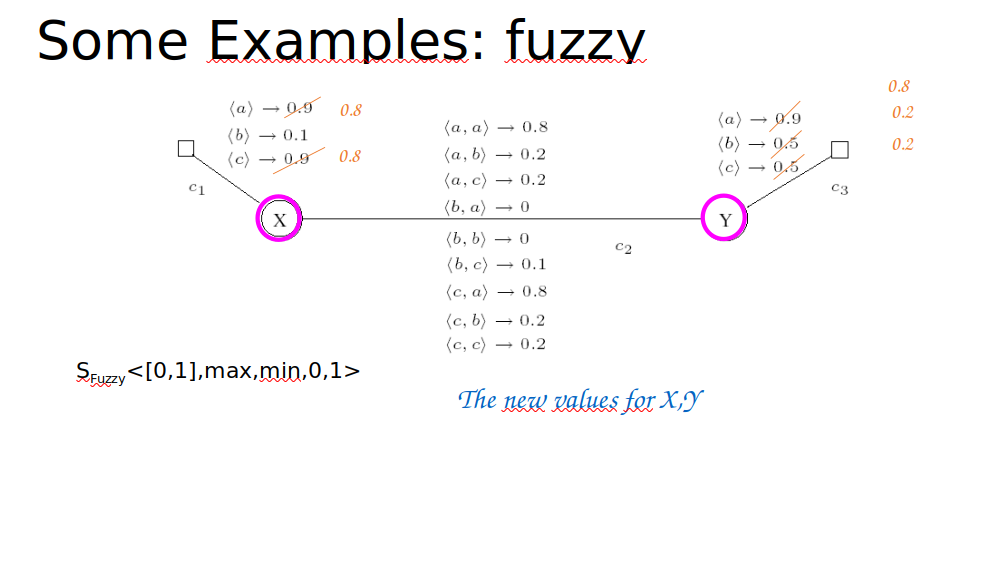
\includegraphics[width=15cm, keepaspectratio]{latex/img/Cap5/ffuzzy2.png}
\end{figure}
Consideriamo il vincolo unario c1 sulla variabile X ed il vincolo binario $c_2$ sulle variabili X ed Y. Faccio $c_1$ $(x)$ $c_2$ proiettato $x(a)$:
\begin{enumerate}
    \item Combinazione (Min): $c_1$ combinato $c_2$ ($c_3$ non lo prendo in considerazione perchè faccio $(x$):
    \begin{itemize}
        \item Quando vale $< a, a >?$ Faccio 0.9 min 0.8 $=$ 0.8
        \item Quando vale $< a, b >?$ Faccio 0.9 min 0.2 $=$ 0.2
        \item Quando vale $< a, c >?$ Faccio 0.9 min 0.2 $=$ 0.2
    \end{itemize}
    Facendo questo ho combinato i vincoli c1 e c2 . Per sapere poi quanto vale $c_1$ $(x)$ $c_2$ devo andare a proiettare su X.
    \item Proiezione (Max): Prendo il massimo tra 0.8, 0.2, 0.2. In conclusione, al posto di 0.9 su (a) posso scriverci 0.8.
\end{enumerate}
\textbf{Altra domanda sul fuzzy (assegnamento): } Quanto vale l’assegnamento $x=a$, $y=b$? 
\\devo fare il minimo tra 0.9, 0.2 e 0.5 che sarebbe 0.2. 
\\(Non applico la proiezione quindi non uso il massimo).
\\Altra domanda: Applichiamo local consistency per X $=$ a.
\\Devo fare min(0.9, 0.8, 0.9) $=$ 0.8.
\\Devo fare min(0.9, 0.2, 0.5) $=$ 0.2.
\\Devo fare min(0.9, 0.2, 0.5) $=$ 0.2.
Se vado a proiettare fa 0.8 perchè prendo il massimo. Se io vado a calcolare la soluzione adesso vado a calcolare la soluzione di '' quanto vale x$=$a y$=$b''?
\\min tra 0.8, 0.2 e 0.2 = 0.2 che è come prima, la soluzione non è cambiata.
\textbf{Ho migliorato il bound ma non ho modificato la soluzione, è una cosa buona.}
\\Nell’ esempio successivo (prossima sezione, sarebbe quello probabilistico) la soluzione \textbf{viene modificata} a 0.72 e non più a 0.9 quindi non posso accettarla, è proprio sbagliata.
\section{Idempotenza degli operatori}
Un operatore si dice idempotente se facendo:
\begin{center}
    a $operazione$ a mi restituisce sempre a.
\end{center}
L’idempotenza si può analizzare sia per gli operatori che si usano per la Proiezione sia per quelli di Combinazione.\\
\begin{itemize}
    \item Idempotenza su \textbf{Combinazione}: Dipende strettamente dal semiring utilizzato:
    \begin{itemize}
        \item \textbf{Fuzzy:} Idempotente, perchè il minimo tra a ed a è sempre a (il minimo tra due valori uguali da sempre lo stesso valore).
        \item \textbf{Probabilistic:} Non idempotente, perchè a $*$ a non fa esattamente a (ad esempio 0.1 $*$ 0.1 $=$ 0.01, la moltiplicazione infatti non ha la proprietà di idempotenza).
        \item \textbf{Weighted:} Non idempotente, perchè a $+$ a non fa esattamente a.
        \item \textbf{Classic:} Idempotente, infatti a and a $=$ a
    \end{itemize}
    \item Idempotenza su \textbf{Proiezione:} Tutti gli operatori sono idempotenti e questo segue dalla definizione stessa di c-semiring (definisco l’ordinamento quando effettuo la proiezione).
\end{itemize}
La distinzione tra operatore idempotente e non idempotente è importante perchè gli algoritmi di consistenza locale solo nel caso in cui la combinazione fosse idempotente \textbf{mantengono le soluzioni del problema}. Qualora facessi arc-consistency su semiring che non ammettono operazioni idempotenti la soluzione che si genera è proprio \textbf{sbagliata}, e non può essere accettata.
\vspace{1cm}

\noindent \textbf{Vediamo un esempio in cui applicare arc-consistency va a modificare la soluzione finale del problema} (e quindi non è accettabile):
\begin{figure}[htp]
	\centering
    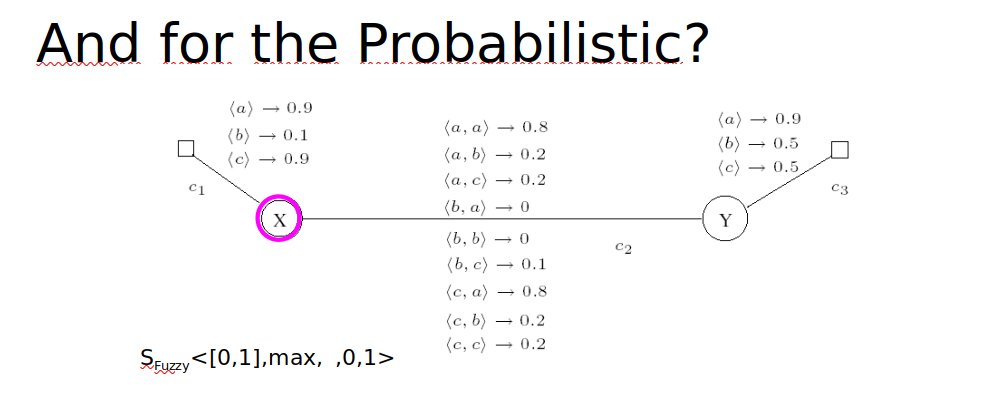
\includegraphics[width=14cm, keepaspectratio]{img/Cap5/probabilistc2.png}
\end{figure}
\\
\textbf{Domanda:} Quanto vale l’assegnamento x $=$ a, y $=$ b su questo problema? 
\\devo moltiplicare 0.9, che sarebbe x$=$a, per $<$ x $=$ a, y $=$ b $>$ che sarebbe 0.2 per y $=$ b che sarebbe 0.5. Il risultato è 0.09.
\\Domanda: Quanto vale c1 c2 proiettato x (su a)? devo fare la combinazione:
\begin{itemize}
    \item 0.9 $*$ 0.8 $=$ 0.72
    \item 0.9 $*$ 0.2 $=$ 0.18
    \item 0.9 $*$ 0.2 $=$ 0.18
\end{itemize}
Poi prendo il Massimo (proiezione) che sarebbe 0.72 e questo valore mi va al posto di 0.9. Il problema però è che ho cambiato la soluzione finale, perchè la proiezione mi ritorna proprio il 0.72 che è un valore errato data la non idempotenza della moltiplicazione (è proprio una soluzione sbagliata).

\vspace{0.8cm}

\noindent L’operazione di local consistency nei CSP Crisp quindi classici è importante perchè mantiene la soluzione del problema riducendo gli elementi del dominio e non modificando le soluzioni.

\vspace{0.5cm}

\noindent Nel caso Soft invece, la soluzione non viene modificata solamente se l’operazione di combinazione è idempotente. Nel caso in cui non lo fosse si andrebbero a modificare le soluzioni stesse del problema, e quest’ultime non sarebbero accettabili perchè sbagliate.

\subsection{Altro esempio con vincolo c3}
\begin{figure}[htp]
	\centering
    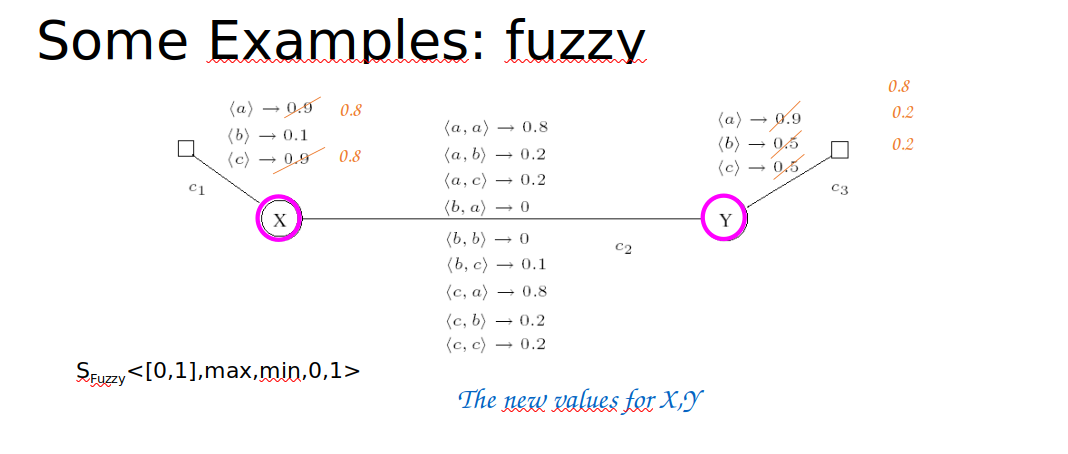
\includegraphics[width=16cm, keepaspectratio]{latex/img/Cap5/FUZZY2.png}
\end{figure}
I nuovi valori per il vincolo c3 sono ottenuti analizzando prima y $=$ a e quindi poi si analizza (a, a) e poi x $=$ a. Poi y $=$ b e quindi poi (b, b) e poi x $=$ b. Utilizzando la combinazione e poi la proiezione i valori tornano quelli.
\subsection{Semiring con operazioni non idempotenti}
\subsubsection{Divisione}
Vogliamo ottimizzare i CSP Soft anche se la loro operazione di combinazione non è idempontente.
\begin{figure}[htp]
	\centering
    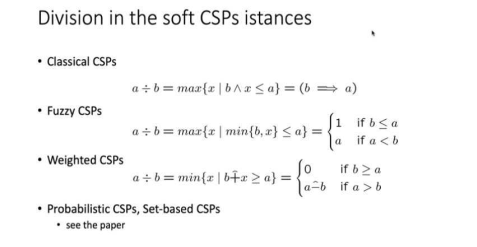
\includegraphics[width=12cm, keepaspectratio]{img/Cap5/DIvisione.png}
\end{figure}
\\L’operatore che utilizzeremo è l’opposto dell’operatore di combinazione ed è chiamato Diviso: $\div$. Analizziamo la riga del Fuzzy:
\begin{itemize}
    \item Prima versione: L’operazione inversa del minimo, indicata con l’operatore $\div$ è max. Supponiamo che l’elemento x sia tale che b $*$ x $=$ a, la domanda è: Quanto fa a $\div$ b? Fa quell’elemento x tale che il minimo tra b ed x è minore uguale di a. Devo quindi in qualche modo andarmi a trovare gli inversi degli operatori visti prima.
    \item  Seconda versione: Quando fa a $\div$ b? (si legge a Diviso b). Fa il numero più grande x tale che il minimo tra b ed x è più piccolo di a
\end{itemize}
Analizziamo la riga del \textbf{Weighted:}
\\Quanto fa a $\div$ b? Fa il più piccolo (min) elemento x tale per cui b $+$ x fa a. Questo però lo possiamo fare solo se a è maggiore di b (altrimenti si prenderebbero in considerazioni valori non consoni tipo negativi) e se b è maggiore uguale di a si da come risultato 0.
\\\textbf{Esempio probabilistico:}
\begin{figure}[htp]
	\centering
    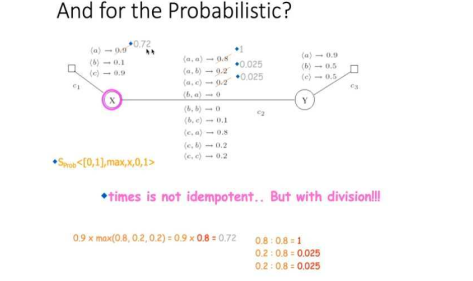
\includegraphics[width=14cm, keepaspectratio]{img/Cap5/Probabilistic2.png}
    % PROBLEMA FOTO
\end{figure}

Come faccio ad ottimizzare il CSP in maniera tale da mantenere le soluzioni?
\\Inizio in maniera identica al precedente metodo:
\begin{itemize}
    \item Combinazione
    \begin{enumerate}
        \item 0.9 * 0.8 = 0.72
        \item 0.9 * 0.2 = 0.18
        \item 0.9 * 0.2 = 0.18
    \end{enumerate}
    \item Proiezione: Max = 0.72
\end{itemize}
\noindent Fatto questo devo \textbf{dividere per il massimo valore tra tutti quelli utilizzati:}
\begin{center}
    $max$(0.8, 0.2, 0.2) = 0.8
\end{center}
Ora divido per 0.8 tutti i valori nel vincolo $c_2$ cosi da ottenere i valori in figura. Dato che ho ottimizzato il valore di (a) e cambiato i valori interessati, la soluzione rimane invariata, quindi anche su semiring non idempotenti si può fare arc-consistency grazie all'operatore di Divisione ($\div$).

\subsubsection{\textbf{Importante}}
In questo caso abbiamo utilizzato la divisione perchè era l'operazione inversa della moltiplicazione (che è l’operatore di combinazione utilizzato nei CSP probabilistici). Se però l’operazione di combinazione fosse stata la Somma (e quindi CSP Weighted) l’operazione $\div$ sarebbe stata la sottrazione.


\chapter{Argumentation Framework} \label{ch:Argumentation Framework}
\section{Argumentation Framework}
Come i CSP l’argumentation è un altro metodo che offre l’intelligenza artificiale per rappresentare la conoscenza e risolvere i problemi. Quello che andremo a rappresentare sono delle situazioni/dialoghi che vogliamo studiare dal punto di vista logico.
\\Argumentation Framework. Un argumentation framework (AF) è una coppia (A,R) dove
\begin{itemize}
    \item A è un set di argomentazioni
    \item R $\subseteq$ A × A è una relazione rappresentante gli "attacchi" ("sconfitte")
\end{itemize}
\begin{center}
    $F(\{a,b,c,d,e\}, \{(a,b),(c,b),(c,d),(d,c),(d,e),(e,e)\})$
\end{center}
\begin{figure}[htp]
	\centering
    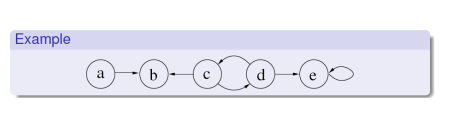
\includegraphics[width=12cm, keepaspectratio]{img/Cap6/arg1.png}
    \caption{Argumentation framework}
\end{figure}
Si ha un attacco quando si ha un’espressione logica (frase, dato...) che è in contraddizione con un’altra. Gli attacchi possono essere anche pesati, essi possono dipendere anche da chi ha detto quella frase.

\begin{figure}[htp]
	\centering
    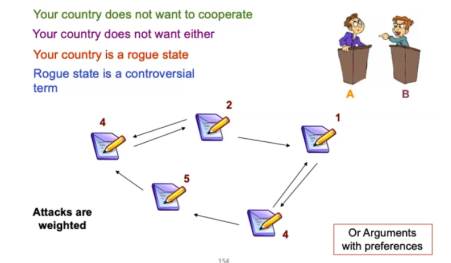
\includegraphics[width=12cm, keepaspectratio]{img/Cap6/arg2.png}
    \caption{Esempio di argumentation framework}
\end{figure}
Ci possono essere anche casi in cui è noto chi dice l’argomento e altri in cui non lo è. Per quest’ultima vogliamo selezionare gli argomenti che sono più validi rispetto agli altri, ad esempio in Figura 6.2 il 4 e il 2 sembrano buoni argomenti perchè attaccano gli altri e contrattaccano nel caso siano attaccati. Lo scopo è di definire dei criteri per trovare gli argomenti più forti, validi (che stanno "in piedi da soli"), in modo da selezione i conflitti che riescono a sopportare gli attacchi dall’esterno.
\begin{figure}[htp]
	\centering
    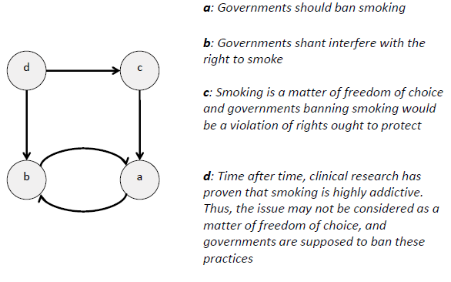
\includegraphics[width=12cm, keepaspectratio]{img/Cap6/arg3.png}
    \caption{Altro esempio di argumentation framework}
\end{figure}
Dobbiamo trovare gli argomenti che "stanno bene insieme", la prima nozione di questo tipo è un insieme di argomenti senza conflitti.

\section{Extension-Based Semantics}
Il task principale che viene svolto sugli argumentation framework è il computo della semantica, cioè si selezionano dei criteri con i quali si vanno a scegliere dei sottoinsiemi di argomenti che condividono una qualche proprietà particolare. La prima che vediamo è quella degli insiemi Conflict Free, cioè quegli insiemi che tra loro non hanno conflitti.
\subsection{Insiemi Conflict Free}
Dato un Augmentation Framework F = (A, R), l’insieme S $\subseteq$ A è conflict-free se, per ogni (a, b) $\in$ S, si ha che (a, b) $\notin$ R. (Per ogni coppia di elementi in S non è presente una relazione d’attacco tra questi elementi).
\begin{figure}[htp]
	\centering
    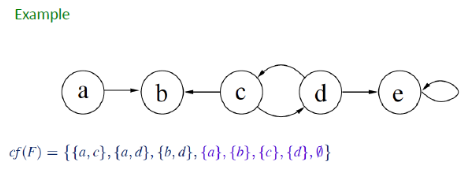
\includegraphics[width=12cm, keepaspectratio]{img/Cap6/cf.png}
    \caption{Esempio insieme conflict-free.}
\end{figure}
\\In questo caso andiamo a scegliere come coppie gli argomenti che non sono in conflitto (quindi che non si attaccano) fra di loro, ({a,c},{a,d} ma non {a,b}), e anche i singoli argomenti tranne e poichè esso si contraddice da solo visto che ha un cappio.

\subsubsection{\textbf{Importante}}
\textbf{Per il calcolo:} Inizio con inserire \textbf{l’insieme vuoto}, poi i \textbf{singoli} argomenti che non si auto-attaccano, poi \textbf{le coppie, terne, quadruple...}

\subsection{Insiemi Ammisibili}
Dato un Augmentation Framework F = (A, R), l’insieme S $\subseteq$ A è ammissibile se:
\begin{itemize}
    \item S è \textbf{conflict free;}
    \item Ogni a $\in$ S è \textbf{difeso} da S (cioè ogni elemento che appartiene all’insieme è difeso dagli elementi dell’insieme stesso). Un elemento a $\in$ A è difeso da S se, per ogni b $\in$ A con (b, a) $\in$ R, esiste un c $\in$ S tale per cui (c, b) $\in$ R (a è difeso da S se per ogni b che attacca quell’elemento a esiste un altro elemento sempre dentro S che contrattacca l’attacco di b verso a).
\end{itemize}
\begin{figure}[htp]
	\centering
    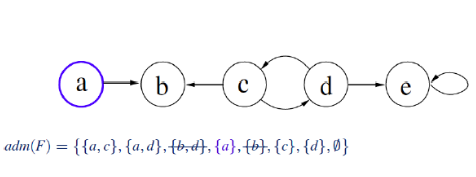
\includegraphics[width=12cm, keepaspectratio]{img/Cap6/ammissibile.png}
    \caption{Esempio insieme Ammisibile.}
\end{figure}
Non è necessario che sia lo stesso argomento a difendersi da altri attacchi, ad esempio in questo caso, supponendo che non ci sia a, b è attaccato da c ma se prendo d lui oltre che difendere se stesso da c (poichè attaccato) difende anche b. Guardando la definizione di difesa, un argomento a è difeso da un argomento b, (b, a) $\in$ R, nel momento in cui esiste un argomento c tale che c attacca b, (c, b) $\in$ R. Il sottoinsieme \{b,d\} non viene scelto poichè d è attaccato da c ma a si difende a sua volta contrattaccando, mentre b è attaccato sia da a che c, nel primo caso nessuno lo difende nel secondo d difende b perchè attacca c.
\begin{itemize}
    \item insieme V vuoto è \textbf{ammissibile}? Si, nessuno lo attacca.
    \item insieme V vuoto è \textbf{Conflict Free}? Si.
\end{itemize}

\subsection{Insiemi Completi (Tutti Difesi)}
Dato un Augmentation Framework F = (A, R), l’insieme S $\subseteq$ A è completo se:
\begin{itemize}
    \item S è ammissibile;
    \item Ogni a $\in$ A difeso da S è contenuto in S. Un elemento a $\in$ A è difeso da S se, per ogni b $\in$ A con (b, a) $\in$ R, esiste un c $\in$ S tale per cui (c, b) $\in$ R.
\end{itemize}
\begin{figure}[htp]
	\centering
    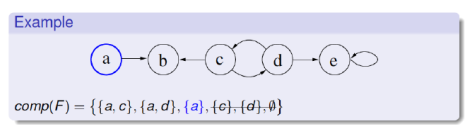
\includegraphics[width=12cm, keepaspectratio]{img/Cap6/completo.png}
    \caption{Esempio insieme Completo.}
\end{figure}
Quindi un insieme complete contiene tutti gli insiemi ammissibili e anche tutti gli argomenti che sono difesi.
\\Insieme V uoto è \textbf{Completo}? Va messo soltanto quando tutti gli argomenti sono attaccati e quindi quando \textbf{non} c’è un qualche argomento che è sempre difeso. 
\\Infatti sopra non va messo perchè a è sempre difeso. a è sempre difeso da tutti perchè non è attaccato da nessuno, quindi nel calcolo dei difensori va sempre messo dentro.
\begin{enumerate}
    \item \{a, c\} è \textbf{completo?} Si!
    \begin{itemize}
        \item a chi difende? attacca b quindi difenderebbe tutti quelli attaccati da b, ma b non attacca nessuno quindi a difende solo se stesso.
        \item c chi difende? tutti quelli attaccati da b quindi nessuno e tutti quelli attaccati da d quindi c.
    \end{itemize}
\textbf{L’insieme dei difensori è a, c, che sta dentro S=\{a, c\}, quindi è completo.}
    \item \{a, d\} è \textbf{completo?}
    \begin{itemize}
        \item a chi difende? attacca b quindi difenderebbe tutti quelli attaccati da b, ma b non attacca nessuno quindi a difende solo se stesso.
        \item d chi difende? se stesso, perchè viene attaccato da c ma si difende da solo con un contrattacco.
    \end{itemize}
    L’insieme dei difensori è \{a, d\} che sta dentro S quindi anche questo è completo.
    \\\{a\} è \textbf{completo?} Può stare da solo perchè non viene attaccato da nessuno, quindi è \textbf{come se venisse difeso da tutti quanti}, e lui non difende nessuno, poichè b non attacca nessuno. 
    \\Quindi se un argomento non attaccato da nessuno ne attacca un altro che a sua volta non attacca nessuno allora quell’elemento è complete e può stare da solo.
    \\\{c\} è \textbf{completo?} Difensori: \{a, c\} che non è incluso in c quindi No.
    \\\{d\} è \textbf{completo?} Difensori: \{a, d\} quindi No. L’idea degli insiemi complete è che se un insieme difende qualcosa, quel qualcosa ”deve essere messo dentro” e \textbf{deve rimanere ammissibile.}
    
    \vspace{0.8cm}
    
    La differenza quindi è che nell’insieme ammissibile vuol dire che mi difendo, complete vuol dire che dentro ci sono tutti quelli difesi.
\end{enumerate}
\
\subsection{Estenzioni Grounded (minimale)}
F = (A, R), l’insieme S $\subseteq$ A è grounded se:
\begin{itemize}
    \item S è \textbf{completo};
    \item Per ogni sotto insieme T $\subseteq$ A completo in F si ha che T $\subsetneq$ S
\end{itemize}
Quindi un insieme completo è grounded se è il \textbf{più piccolo dei complete}, ovvero se \textbf{non} esiste un sottoinsieme T complete che è più piccolo di lui. Si calcola tramite \textbf{l’intersezione} delle complete.
\textbf{N.B} L’insieme grounded è sempre \textbf{UNICO}, cioè composto da un solo elemento.
\begin{figure}[htp]
	\centering
    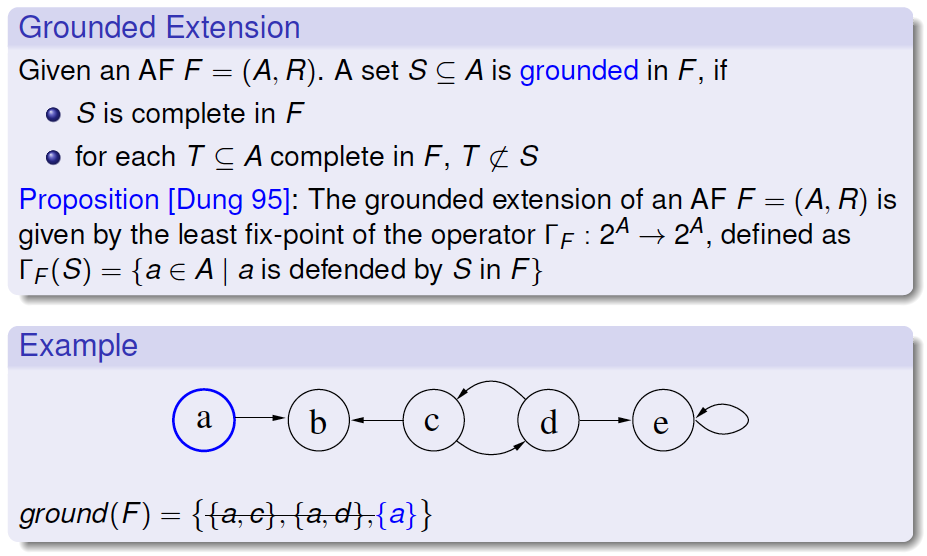
\includegraphics[width=12cm, keepaspectratio]{latex/img/Cap6/grounded.png}
    \caption{Esempio Grounded} 
\end{figure}
\\a, c è \textbf{grounded}? i suoi sottoinsiemi singoli sono a e c, questi sono completi?
\\no, perchè a lo è ma non c quindi non è grounded.
\\a, d è \textbf{grounded}? i suoi sottoinsiemi singoli sono a e d, questi sono completi?
\\no, perchè a lo è ma non d quindi non è grounded.
\\a è \textbf{grounded}? Si, i suoi sottoinsiemi singoli sono a ed è completo.

\vspace{0.8cm}

\textbf{N.B} L’insieme grounded è dato anche dall’intersezione di tutti gli insiemi completi, infatti sopra se intersechiamo quei 3 insiemi completi l’unica cosa che viene fuori era a che infatti è l’unico insieme grounded.

\subsection{Estenzioni Preferred (massimale)}
Dato un Augmentation Framework F = (A, R), l’insieme S $\subseteq$ A è preferred se:
\begin{itemize}
    \item S è ammissibile;
    \item Per ogni sotto insieme T $\subseteq$ A ammissibile in F , si ha che S $\subsetneq$ T (cioè se nessuno degli ammissibili S è più grande di T).
\end{itemize}
\begin{figure}[htp]
	\centering
    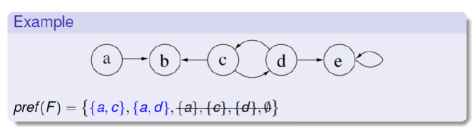
\includegraphics[width=12cm, keepaspectratio]{img/Cap6/prefered.png}
    \caption{Esempio Preferred}
\end{figure}
Si ottiene per inclusione insiemistica, \textbf{Le più grandi delle admissible}. (a) da solo è contenuto in (a,c) che è più grande quindi sicuramente non sarà preferred, stessa cosa per (d). (c) stessa cosa per (a,c).
\\Al contrario di grounded dove si andava a scegliere l’insieme con l’elemento in
comune con gli altri insieme, in questo caso si va a scegliere tra gli insiemi ammissibili
quelli che sono più grandi. Da notare che si sceglie tra gli insiemi ammissibili ma si
può dimostrare che si può scegliere da quelli complete.

\subsection{Estenzioni Stable}
Dato un AF, F=(A,R). Un insieme S $\subseteq$ A è stabile in F, se
\begin{itemize}
    \item S è \textbf{conflict-free} in F
    \item per ogni a $\in$ A / S, esiste una b $\in$ S, tale che (b, a) $\in$ R.
\end{itemize}
\begin{figure}[htp]
	\centering
    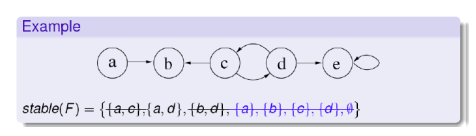
\includegraphics[width=12cm, keepaspectratio]{img/Cap6/stable.png}
    \caption{Esempio Stable}
\end{figure}
Per ogni elemento fuori da S esiste un elemento di S che lo attacca. Questo significa che gli insiemi stable sono gli insiemi conflict-free che attaccano tutti gli altri, ovvero che tutti gli elementi che stanno fuori dall’insieme esaminato sono attaccati.\\
In questo caso si sceglie l’insieme i quali elementi attaccano tutti gli elementi fuori dall’insieme conflict-free, ad esempio \{a,c\} non si prende perchè a attacca b e c attacca d e b ma nessuno dei due attacca e. Mentre nell’insieme \{a,d\} a attacca b e d attacca sia c che e. Esiste anche una semantica semi-stabile la quale nel caso cui esista un insieme stabile allora essa coincide con quest’ultimo ma quando non c’è la stabile allora sceglie tra gli insieme preffered quelli che ne attaccano di più tra gli insiemi fuori a quest’ultimo. L’obiettivo della semantica stabile è di avere cardinalità più grande possibile e di attaccare tutti gli insiemi fuori.

\vspace{0.5cm}

\noindent a, c \textbf{non è stabile} perchè è si ammissibile (b che sta fuori è attaccato e ok), d sta fuori ed è attaccato, ma e non lo attacca ne a ne c quindi questo insieme non può essere stabile.
\\a, d \textbf{è stabile} perchè a attacca b e d attacca c, e quindi tutti gli elementi fuori dall’insieme sono attaccati.
\\La semantica stabile è la più forte di tutte le estenzioni, perchè sono le posizioni più forti in un dialogo, sono la scelta migliore quando utilizzo AF come decision making. Il problema delle estenzioni stabili è che non sempre esistono.

\section{Soft Argumentation Framework (Weighted AF)}
Un Soft Argumentation Framework è una quadrupla:
\begin{center}
    $(A_{rgs} , R, W, S)$
\end{center}
dove:
\begin{itemize}
    \item $A_{rgs}$ è un insieme di Argomenti.
    \item R è una relazione di attacco sugli argomenti in $A_{rgs}$.
    \item W : $A_{rgs}$ x $A_{rgs}$ $\rightarrow$ S è una funzione binaria che rappresenta il peso associato ad ogni arco.
    \item S è un semiring $< A, +, x, bottom, top >$ Dati a, b $\in$ Args , $\forall$(a, b) $\in$ R, W (a, b) = s significa che a attacca b con un peso di s $\in$ S.
\end{itemize}
\newpage
\textbf{ Esempio:}
\begin{figure}[htp]
	\centering
    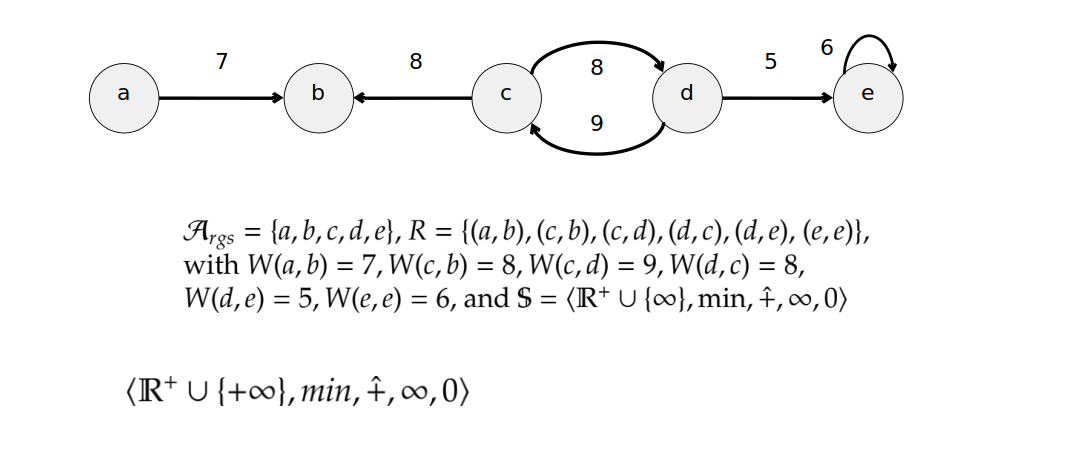
\includegraphics[width=14cm, keepaspectratio]{latex/img/Cap6/SoftA2.png}
\end{figure}
\\\textbf{Cambia la nozione di attacco:} Prima l’attacco era una funzione booleana (a attacca b). Adesso invece quando a attacca b gli viene associato un valore (comunque appartenente al semiring).
\\\textbf{Cambia la nozione di difesa:} Nell’esempio sopra, nel caso in cui fossimo negli AF tradizionali C si difenderebbe dall’attacco di D (perchè ricordiamo era una funzione booleana). In questo caso però, essendo che d attacca c con 9 e c risponde con 8, c non potrà difendersi dall’attacco, poichè la difesa non è sufficiente a contrastare quest’ultimo. Questa nozione dipende strettamente dal semiring utilizzato, poichè per ogni semiring (i cui tipi sono gli stessi introdotti precedentemente) si avranno relazioni diverse.
\subsection{w-difesa (Dw)}
Dato un Soft Argumentation Framework $(A_{rgs} , R, W, S)$, un sottoinsieme di argomenti B $\subseteq$ Args w-difende un argomento b $\in$ Args se e soltanto se, dato a $\in$ Args tale per cui R(a, b), allora:
\begin{center}
    $W (a, B \cup \{b\}) >=_s s W (B, a)$
\end{center}
L’insieme B w-difende l’elemento b se e soltanto se difende b da tutti gli attacchi che arrivano a b cioè da tutti gli R(a, b).
\\$>=_S$ è da intendere come elemento migliore o peggiore all’interno del semiring.
\\In altre parole, devo verificare che il peso degli attacchi che ricevo sia inferiore al peso degli attacchi che invio.
\begin{itemize}
    \item Con W (a, B $\cup$ \{b\}) si intende il costo degli attacchi che vanno da a all’insieme B $\cup$ \{b\} (cioè tutti gli attacchi che apporta quell’elemento a all’insieme B "dall’esterno verso l’interno") sommati con l’operatore di combinazione del semiring. Per sapere quindi quanto vale l’attacco di a verso l’insieme B $\cup$ \{b\} nel caso di Semiring Weighted ad esempio devo fare la somma di tutti gli attacchi (proprio perchè l’operatore di combinazione è la somma).
    \item W (B, a) sarebbe "con quanto l’insieme B attacca a, cioè tutti gli attacchi dall’interno di B all’esterno". Anche questo dipende strettamente dal semiring, nel Weighted vanno tutti sommati.
\end{itemize}
\textbf{Esempio}
\begin{figure}[htp]
	\centering
    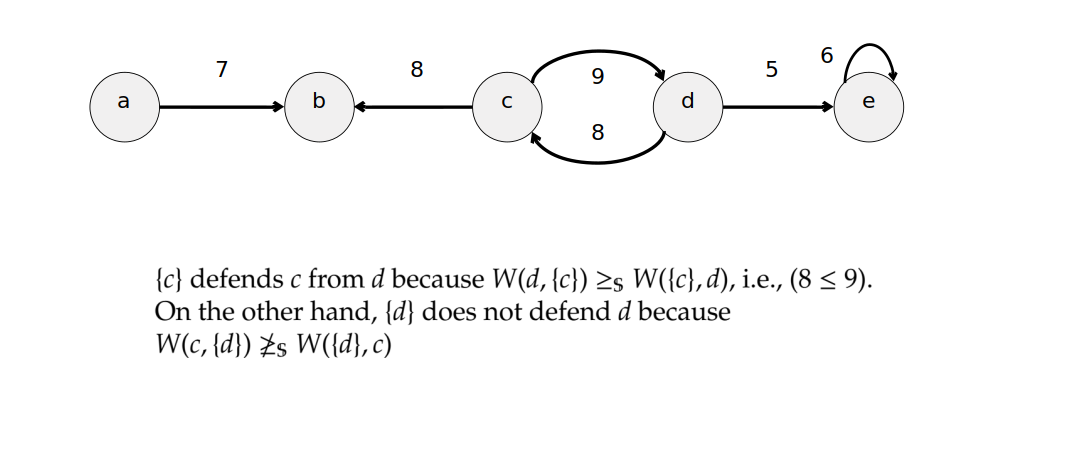
\includegraphics[width=14cm, keepaspectratio]{latex/img/Cap6/srs2.png}
\end{figure}
\\Per il calcolo degli insiemi ammissibili esistono vari metodi, che variano in base a regole imposte da autori di articoli scientifici.

\subsection{Semantiche nei Weighted AF (W AAFs)}
\subsubsection{w-Conflict Free}
Dato un W F = $(A_{rgs} , R, W, S)$, un sottoinsieme di argomenti B $\subseteq$ Args è w-conflict free se e soltanto se W(B, B) = top (top del semiring). Questo significa che nessuno degli elementi dentro l’insieme attacca un altro elemento sempre dentro l’insieme. Dire che il peso è uguale al top del semiring (o al bottom) significa che quel peso non è presente, e quindi non è presente una relazione di attacco.
\subsubsection{w-Admissible}
Dato un W F = $(A_{rgs} , R, W, S)$, un insieme di argomenti B $\subseteq$ Args w-conflict-free è w-admissible se e soltanto se tutti gli argomenti di B sono w-difesi da B.
\section{Distinzione tra gli insiemi Admissible}
\subsection{Martinez e Simari (D1)}
L’obiettivo è capire se l’insieme B = \{b, c, d, e\} riesce a difendersi dall’attacco di a e poi dall’attacco di f , cioè se quell'insieme è ammissibile. Prendiamo in considerazione per tutti il semiring Weighted. Secondo Martinez e Simari non si aggregano ne le difese ne gli attacchi, quindi prendo il massimo degli attacchi ed il massimo delle difese.
\begin{figure}[htp]
	\centering
    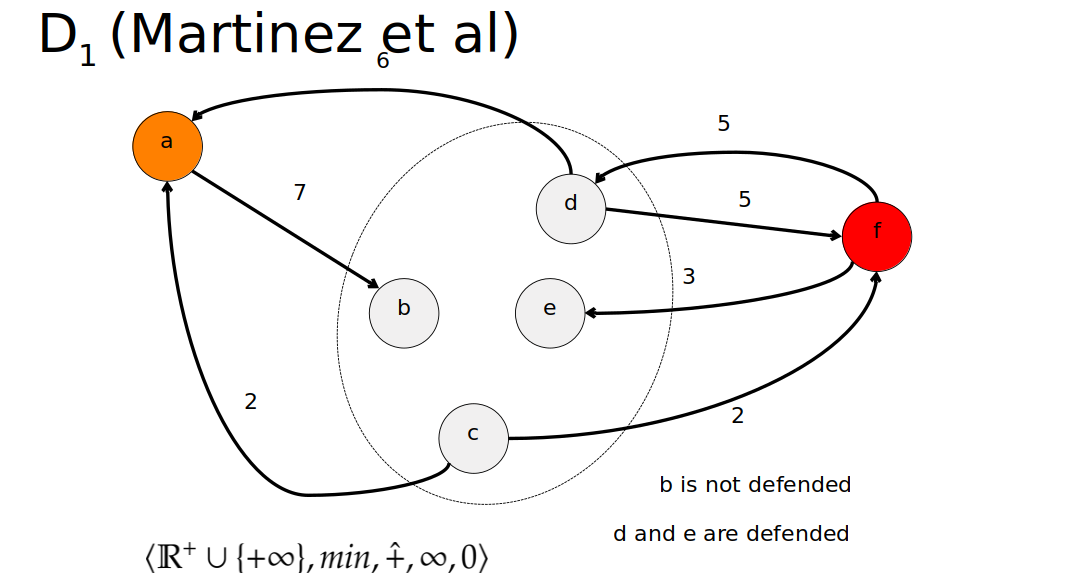
\includegraphics[width=13cm, keepaspectratio]{img/Cap6/martinez2.png}

\end{figure}
\\\textbf{Esempio:} Devo verificare che il \textbf{massimo} valore degli \textbf{attacchi} sia maggiore del \textbf{massimo} valore delle \textbf{difese}.
\\\textbf{Attacco} di a \textbf{verso} b:
\begin{itemize}
    \item Attaccanti (a): Max(7) = 7
    \item Difensori (d,c): Max(6,2) = 6
    \item Conclusione: 6 $<$ 7, b non è difeso e quindi non ammissibile
\end{itemize}
\textbf{Attacco} di f \textbf{verso} d, e:
\begin{itemize}
    \item  Attaccanti (f): Max(5,3) = 5
    \item Difensori (d,e): Max(5,2) = 5 (il 2 viene dall’attacco di c verso f)
    \item Conclusione: 5 = 5, (d), (e) sono difesi e quindi ammissibili.
\end{itemize}
La nozione formale di difesa in Simari-Martinez è: Dato W F = $(A_{rgs} , R, W, S)$, a, b, c $\in$ $A_{rgs}$ , B $\subseteq$ $A_{rgs}$ , allora b è difeso da B se per ogni R(a, b), esiste almeno uno c $\in$ B tale per cui W (a, b) $>=_s$ W (c, a).


\subsection{Coste-Marquis (D2)}
Questo approccio aggrega solamente le \textbf{difese.}
\begin{figure}[htp]
	\centering
    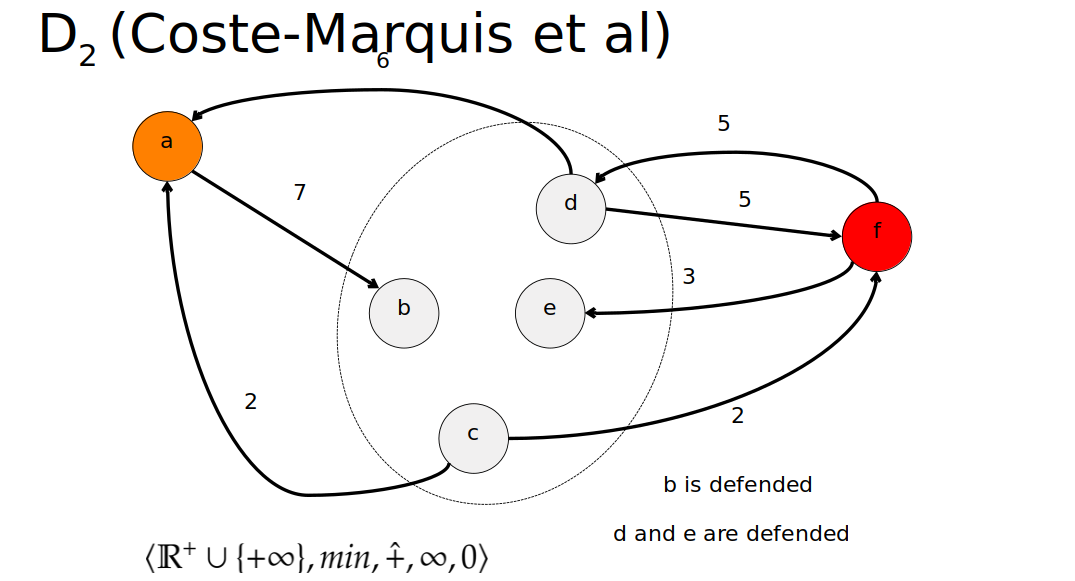
\includegraphics[width=13cm, keepaspectratio]{latex/img/Cap6/marquis2.png}
\end{figure}
\\\textbf{Attacco} di a \textbf{verso} b:
\begin{itemize}
    \item Attaccanti (a): Max(7) = 7
    \item Difensori (d,c): Difesa(6)+Difesa(2) = 6+2 = 8
    \item Conclusione: 8 $>$ 7, b è difeso e quindi ammissibile
\end{itemize}

\subsection{Santini e Bistarelli (Dw)}
Questo approccio aggrega \textbf{sia gli attacchi che le difese, ciò vuol dire che b è difeso ma d ed e no.}

\begin{figure}[htp]
	\centering
    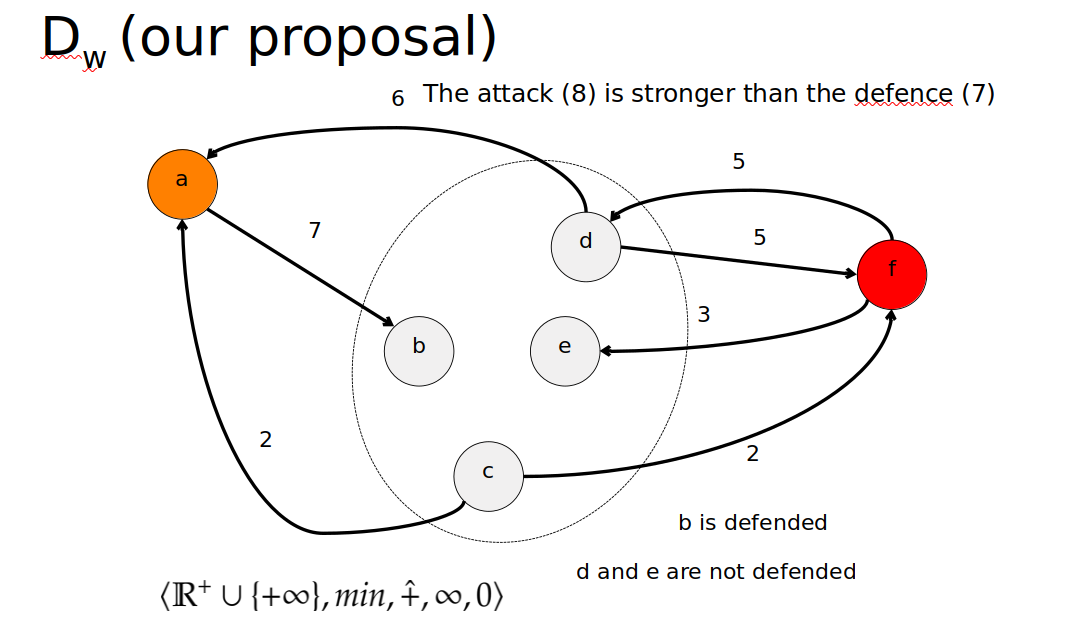
\includegraphics[width=13cm, keepaspectratio]{img/Cap6/bistarelli2.png}
\end{figure}

\textbf{Attacco} di a \textbf{verso b:}

\begin{itemize}
    \item Attaccanti (a): Attacco(7) = 7
    \item Difensori (d,c): Difesa(6)+Difesa(2) = 6+2 = 8
    \item Conclusione: 8 $>$ 7, b è difeso e quindi ammissibile
\end{itemize}
\textbf{Attacco} di f \textbf{verso d, e:}
\begin{itemize}
    \item Attaccanti (f): Attacco(5)+Attacco(3) = 5+3 = 8
    \item Difensori (d,e): Difesa(5) + Difesa(2) = 7
    \item Conclusione: 8 $>$ 7, d, e \textbf{non} sono difesi e quindi non ammissibili.
\end{itemize}

\newpage
\section{Teoremi di implicazione tra le nozioni}
\textbf{N.B1 (da sapere):} La relazione di w-difesa implica la relazione di difesa:
\begin{center}
    B w-difende b $\rightarrow$ B difende b
\end{center}
\textbf{N.B2:} Nel semiring Classic (booleano) si ha che:
\begin{center}
    B w-difende a $\Leftarrow \Rightarrow$ B difende a
\end{center}
\begin{itemize}
    \item $D_W$ $\Rightarrow$ $D_2$ , Bista implica Costa-Marquis
    \item $D_1$ $\Rightarrow$ $D_2$ , Martinez implica Costa-Marquis
    \item Quindi se è ammissibile per Martinez e Bista allora è ammissibile anche per Costa-Marquiz
    \item Se S $=< [0, 1], max, min, 0, 1 > $ cioè semiring Fuzzy, allora D1 $\Leftarrow \Rightarrow$ D2
    \item Se $S =< [0, 1], max, min, 0, 1 >$ cioè semiring Fuzzy, allora Dw $\Leftarrow \Rightarrow$ D1
    \item Se $S =< [true, false], or, and, false, true >$ cioè semiring Classic, 
    \\allora $D_w \Leftarrow \Rightarrow D_0 \Leftarrow \Rightarrow D1 \Leftarrow \Rightarrow D_2$ (ma cosa è $D_0$ )??
\end{itemize}
\begin{figure}[htp]
	\centering
    \includegraphics[width=12cm, keepaspectratio]{img/Cap6/teor1.png}
    \includegraphics[width=12cm, keepaspectratio]{img/Cap6/teor2.png}
\end{figure}
L’implicazione delle semantiche è la stessa sia nel caso classico che in quello pesato.
\newpage
\section{Orthogonal Relaxations}
\begin{figure}[htp]
	\centering
    \includegraphics[width=12cm, keepaspectratio]{img/Cap6/ortogonal.png}
\end{figure}
\noindent In questo esempio notiamo che (d, c) non stanno bene insieme, perchè si attaccato 100. (b, c) sono abbastanza compatibili, perchè la relazione di attacco è presente ma con peso molto basso. Abbiamo poi che b non è ammissibile (non riesce a difendersi da c), c è ammissibile, d è ammissibile e nessuna
coppia di argomenti è ammissibile. Questo però non è una cosa positiva, perchè si vorrebbero cercare delle coalizioni superiori al singleton. Se però riuscissi ad accettare un po’ di conflitti interni potrei comunque creare una coalizione. Infatti notiamo che potremmo mettere insieme (b, c) dato che
la relazione di attacco è si presente ma con peso molto basso. Introduciamo quindi l’Alpha-hamma consistenza.\\
Questi rilassamenti sono strettamente correlati
e influenzano l’un l’altro: permettere un piccolo conflitto può portare ad avere più
argomentazioni in un’estensione, e di conseguenza si ha una difesa più forte o più debole.
Un esempio reale potrebbe essere in campo politico, partiti con piccole divergenze
interne si uniscono in modo da raggiungere una percentuale sufficiente di voti per
governare.

\section{Alpha-Gamma consistenza}
Che cosa è l’\textbf{alpha-gamma consistenza?}
\\ Questa consistenza definisce il quantitativo di attacchi "interni" cioè alpha ed ”esterni” cioè gamma che si ammettono.
\begin{figure}[htp]
	\centering
    \includegraphics[width=12cm, keepaspectratio]{img/Cap6/cons2.png}
\end{figure}
\\In questo esempio, l’insieme $B = \{b, c, d, e\}$ non è conflict-free (b e d attaccano e), però se volessimo misurare il valore di questo conflitto considerando il semiring Weighted (operazione somma), l’insieme è 2-conflict-free (infatti 2 elementi in questo insieme attaccano un altro elemento sempre appartenente all’insieme). Se quindi la soglia $\alpha$ fosse 2 riuscirei a sopportare l’attacco
tramite il rilassamento dei conflitti interni. Guardiamo l’ammissibilità dell’insieme: a attacca l’insieme B con 5 e B è difeso da 1 ed 1. In realtà l’argomento d andrebbe escluso dall’insieme
perchè porta un attacco con peso molto alto all’insieme stesso. Se però devo per forza costruire un organo di 4 elementi devo accettare sia i conflitti interni sia l’attacco verso d (potrei anche portare dentro a).

\subsubsection{Unità di sopportazione $\gamma$}
\textbf{N.B} secondo Bistarelli l’insieme B non è ammissibile, perchè l’attacco di 5 non è difeso dalla somma delle difese 1+1=2. Facendo il calcolo: (attacco-difesa) 5-2=3 si calcola l’unità di \textbf{sopportazione} $\gamma$ che in questo caso è 3.
\\Quindi:
\begin{itemize}
    \item $\alpha$ Peso del \textbf{conflitto interno} (in questo caso 2, dall’attacco di b pari ad 1 e d sempre 1 verso e)
    \item $\gamma$ Peso del \textbf{conflitto esterno} (in questo caso 3 (5 - 2))
\end{itemize}
L’insieme dell’esempio sopra è $2^3$ \textbf{admissible} perchè $\alpha$ = 2 e $\gamma$ = 3. Inoltre B è anche stabile, perchè tutti gli elementi esterni (in questo caso solo a) sono attaccati. Nel caso in cui portassimo d fuori si avrebbe un valore più basso di $\gamma$ ma B non sarebbe stato stabile, perchè nessuno attaccava d (a rimaneva comunque fuori).
\\
La semantica Alpha Gamma può essere descritta come:
\begin{center}
    $W (a, B \cup \{b\}) \div W (B, a)) >=_s \gamma$
\end{center}
dove:
\begin{itemize}
    \item $W (a, B \cup \{b\})$ : Il peso dell’attacco dall’esterno a verso l’interno B
    \item $\div$ : opposto della combinazione (x), abbiamo fatto esempi sempre con il Weighted, cioè la somma, quindi assumiamo sia la \textbf{sottrazione}
    \item W (B, a) Il peso dell’attacco dall’interno B verso l’esterno a
    \item Il risultato deve essere $>=_s$ $\gamma$ (migliore all’interno del semiring s).
\end{itemize}
L’insieme $B = \{b, c, d, e\}$ è anche $4^5$ \textbf{admissible}, e per dimostrare questo facciamo riferimento alle inclusioni.

\subsection{Inclusioni in Alpha-Gamma consistenza}
\textbf{Teorema}: Dato un W F=$(A_{rgs }, R, W, S)$ con S=$(A, (+), (x), bottom, top)$ e $\alpha, \gamma \in$ A:
\begin{center}
    $\alpha^\gamma-stable \rightarrow \alpha^\gamma-prefered \rightarrow \alpha^\gamma-complete \rightarrow \alpha^\gamma-admissible \rightarrow \alpha-conflict-free$
\end{center}
\begin{figure}[htp]
	\centering
    \includegraphics[width=15cm, keepaspectratio]{latex/img/Cap6/alpha-gamma2.png}
\end{figure}
\textbf{Le uniche cose spiegate dal prof nella figura sopra sono:}
\\Se un estenzione è $ \alpha_1$ ammissibile e $\alpha_1 >=_s \alpha_2$ allora quell’estenzione è anche $\alpha_2$ ammissibile. Stessa cosa per $\gamma$.
\\Questo significa che nell’esempio sopra che era $2^3$ admissible sarà anche $4^5$ ammissibile (ecco spiegata la domanda della sezione sopra).

\section{Semantica w-Grounded}
Gli insiemi grounded sono gli insiemi complete più piccoli.
\\\textbf{Def di Grounded (Minimale) nel caso normale (Crisp AF):}
\begin{center}
    E $\in$ gr(F) if f E $\in$ co(F) e \textbf{non esiste} E' $\in$ co(f) tale per cui E' \textbf{non è contenuto} in E.
\end{center}
Un estenzione E è grounded se e solo se è una complete e nessun altra estenzione dentro le complete è più piccola di lei (quindi è la più piccola delle complete).
\begin{figure}[htp]
	\centering
    \includegraphics[width=12cm, keepaspectratio]{img/Cap6/w-grounded.png}
\end{figure}
\\\textbf{Calcolo delle complete se non ci fossero i pesi:} L’insieme complete era (a, d, c) perchè a difendeva sia d che c insieme. 
\\\textbf{Calcolo delle complete con pesi (usiamo Bistarelli):} Le complete in questo caso sono a perchè non viene attaccata da nessuno e più tutte quelle difese da a cioè d e c. \textbf{Non le difende tutte e due insieme} perchè il costo 1 non è sufficiente e difenderle tutte e due, deve per forza farlo uno alla volta (cosi ha detto il bista). Quindi le complete sono (a, d) e (a, c). Applicando la definizione di Grounded all’esempio otteniamo che l’insieme è sempre lo stesso delle complete, ma questo è un problema, perchè le grounded hanno la proprietà di essere \textbf{uniche}.
\\\textbf{Tutto quello sopra è per dimostrare che la definizione di Grounded con pesi negli AF va cambiata a}:\\
Un elemento E è Grounded se e soltanto se:
\begin{enumerate}
    \item \textbf{ É ammissibile} (prima si richiedeva che era complete);
    \item  É incluso nell’intersezione delle \textbf{complete};
    \item  Non esiste nessun elemento \textbf{ammissibile} più grande di E.
\end{enumerate}
\begin{figure}[htp]
	\centering
    \includegraphics[width=12cm, keepaspectratio]{img/Cap6/w-gounded2.png}
\end{figure}
L’insieme degli ammissibili in questo caso era: (a), (a, c), (a, d) quindi l’intersezione viene a che è appunto l’unica grounded (e non è attaccata da nessuno).
\\Negli Weighted AF la definizione di Grounded va cambiata perchè altrimenti si perderebbe la proprietà di essere \textbf{uniche}.
\section{Argomento Scetticamente/Credulosamente accettato}
Trattiamo adesso un problema decisionale (quindi chiedere se un argomento è SI/NO), introducendo il significato di un argomento Credulosamente o \textbf{Skep/(Scet)ticamente }accettato su questo esempio.
\begin{figure}[htp]
	\centering
    \includegraphics[width=12cm, keepaspectratio]{img/Cap6/scet.png}
\end{figure}
\begin{itemize}
    \item \textbf{Cred} (Almeno in un insieme): Ci domandiamo: esiste \textbf{almeno} una volta che l’argomento 2 compare in output? La domanda va posta in base a quello che calcoliamo, ad esempio, nel caso in cui calcolassimo le conflict-free e il 2 non compare tra le coppie che lo sono, la risposta sarà NO, mentre nel caso in cui comparisse in almeno una coppia (o anche da solo) la risposta sarebbe SI.
    \item \textbf{Skept} (In tutti gli insiemi): Se un elemento è \textbf{sempre} dentro un estenzione. In questo caso l’output sarà NO perchè non c’è un elemento che è comune a tutti gli insiemi. É possibile selezionare l’elemento, quindi magari per il valore 4 da NO, ma per il valore 3 da SI.
\end{itemize}

\section{Tipologie di semantiche}
Esistono principalmente tre tipologie di semantiche basate sulla metodologia
con la quale vengono calcolate.
\begin{enumerate}
    \item \textbf{Estensione:} Andiamo a guardare dei sottoinsieme di argomenti (tutte quelle viste precedentemente)
    \item \textbf{Labeling:} Il labeling è una funzione che assegna delle etichette (colori) ad ogni argomento in modo tale da distinguere gli argomenti accettati dai restanti.
    \item \textbf{Ranking:} Restituisce un ordimento sugli argomenti. Dice quindi "l’argomento a è migliore di b". Questo sistema è più raffinato.
\end{enumerate}
\section{Semantiche basate su Estensione (ripetizione)}
\begin{itemize}
    \item \textbf{Conflict Free}: Argomenti che non si attaccano.
    \item \textbf{Ammissible}: Richiede la nozione di difesa, cioè un contrattacco che un argomento fa ad un altro argomento che è attaccato.
    \item \textbf{Complete}: Deve essere admissible, se un argomento è difeso questo è per forza dentro l’estenzione. Nell’esempio sopra a era l’unico argomento che era sempre difeso (non veniva attaccato da nessuno) quindi l’insieme complete sono tutti gli argomenti che hanno dentro a.
    \item \textbf{Prefered}: Si ottiene per inclusione insiemistica, cerco le admissible più grandi. tra \{a\},\{c\},\{d\},\{a, c\},\{a, d\} dato che voglio la più grande, la singola {a} non potrà essere prefered, perchè si trova dentro \{a, c\},\{a, d\} che sono più grandi.
    \item \textbf{Grounded}: Set più piccolo tra tutte le complete.
    \item \textbf{Stable}: Seleziono un insieme di argomenti che è conflict free e che attacca tutti gli altri
\end{itemize}

\chapter{Semantiche basate su Labelling} \label{ch:Semantiche basate su Labelling}
\section{Semantiche basate su Labelling}
Il Labeling è una funzione che assegna delle etichette rappresentate come colori ad ogni argomento. Le etichette sono di tre tipi:
\begin{enumerate}
    \item \textbf{Verdi:} Corrispondono ad argomenti IN, cioè sono ”dentro” l’insieme di argomenti accettati.
    \item \textbf{Rosse:} Corrispondono ad argomenti OUT, cioè sono ”fuori” dall’insieme di argomenti accettati.
    \item \textbf{Gialle:} ”Undecided” e sono fuori dagli insiemi direttamente accettati(verdi) ma non sono direttamente Rejected (rossi), ovvero non ho una motivazione esplicita per non accettare quel nodo, quindi sono una via di mezzo.
\end{enumerate}
Qualsiasi assegnamento di colori è un labeling (posso colorare tutti i nodi di verde e apposto), però chiaramente non rispetterà le semantiche che adesso introdurremo. Le semantiche basate su labeling corrispondono esattamente alle semantiche basate su estenzioni, ed infatti possiamo calcolare le stesse
cose.

\subsection{Conflict-Free Labeling Based}
Per ogni argomento $a \in A$ si ha che:
\begin{itemize}
    \item $a$ è \textbf{IN} se non ha altri attaccanti IN.
    \item $a$ è \textbf{OUT} se è attaccato da almeno un argomento IN.
\end{itemize}
\begin{figure}[htp]
	\centering
    \includegraphics[width=12cm, keepaspectratio]{img/Cap7/CF.png}
    \caption{Esempio di Conflict-Free Labeling.}
\end{figure}
\begin{itemize}
    \item $a$ è verde perchè non ha nessun altro argomento verde che lo attacca.
    \item $c$ è verde per lo stesso motivo
    \item $b$ e $d$ sono rossi perchè c’è almeno un argomento verde che li attacca.
    \item $e$ è attaccato da un argomento rosso, ma le regole non specificano il colore in questo caso, quindi l’argomento resta fuori sia dalla colorazione IN che OUT. Per esprimere questa incertezza utilizzo la label gialla.
\end{itemize}
\textbf{Domanda: } Questo labeling sotto è conflict free? (cioè soddisfa le regole scritte sopra?)
\begin{figure}[htp]
	\centering
    \includegraphics[width=12cm, keepaspectratio]{img/Cap7/CF2.png}
    \caption{Conflict free label}
\end{figure}
\begin{center}
    \textbf{Si, nessuna regola viene violata.}
\end{center}

\textbf{Domanda: } Questo labeling sotto è conflict free?
\begin{figure}[htp]
	\centering
    \includegraphics[width=12cm, keepaspectratio]{img/Cap7/CF3.png}
    \caption{No conflict free label}
\end{figure}
\begin{center}
    \textbf{No! perchè a è rosso ma non ha un argomento verde che lo attacca.}
\end{center}
\newpage
\subsection{Labeling Admissible}
Per ogni argomento $a \in A$ si ha che:
\begin{itemize}
    \item $a$ è \textbf{IN} se tutti i suoi attaccanti sono OUT.
    \item $a$ è \textbf{OUT} se è attaccato da almeno un argomento IN. In questo caso c’è la nozione di Difesa, ovvero che un argomento è accettato (è IN) solamente se tutti i suoi attaccanti sono sconfitti (OUT)
\end{itemize}
In questo caso c’è la nozione di Difesa, ovvero che un argomento è accettato (è IN) solamente se \textbf{tutti} i suoi attaccanti sono sconfitti (OUT)
\begin{figure}[htp]
	\centering
    \includegraphics[width=12cm, keepaspectratio]{img/Cap7/LA.png}
    \caption{Esempio Labeling Admissible}
\end{figure}
\\Questo labeling è admissible, ad esempio c è accettato perchè d che lo attacca è sconfitto, cioè OUT.
\begin{figure}[htp]
	\centering
    \includegraphics[width=12cm, keepaspectratio]{img/Cap7/LA2.png}
    \caption{Esempio2 Labeling Admissible}
\end{figure}
Questo esempio è comunque admissible, perchè non ho obblighi sull’argomento a, posso etichettarlo di Verde e la regola sarebbe soddisfatta, ma non avendo attaccanti posso etichettarlo sia giallo che verde e non violo nessuna regola.

\subsubsection{\textbf{Differenza}}
La differenza tra Admissible e Complete è che A in complete deve essere per forza verde mentre qui può essere anche giallo.
\newpage
\subsection{Labeling Complete}
Per ogni argomento $a \in A$ si ha che:
\begin{itemize}
    \item  $a$ è \textbf{IN} $se e solo se$ tutti i suoi attaccanti sono etichettati come OUT o quell’argomento non ha attaccanti.
    \item $a$ è \textbf{OUT} $se e solo se$ è attaccato da almeno un argomento IN.
\end{itemize}
\textbf{Domanda: } Questo labeling è complete?
\begin{figure}[htp]
	\centering
    \includegraphics[width=12cm, keepaspectratio]{img/Cap7/LC.png}
    \caption{Esempio Labeling NON COMPLETE}
\end{figure}
\\No, perchè l’argomento a è etichettato di giallo, ma la prima regola mi dice che un argomento è etichettato di verde quando tutti i suoi attaccanti sono etichettati di rosso, ma ho un se e solo se, devo leggerlo anche dalla parte opposta, ovvero:

\vspace{0.3cm}
\noindent É IN se ha tutti attaccanti etichettati OUT, ma dato che a non ha attaccanti deve per forza essere verde, cosi come d.

\vspace{0.3cm}

\noindent \textbf{La differenza} con l’admissible è proprio quel ”se e solo se”. L’admissible ci permette di ignorare degli elementi che potrebbero essere accettati (infatti posso sia etichettarlo verde o giallo a prima), ma questo non accade nella complete, cioè se tutti gli argomenti che mi attaccano sono out (e questo
accade anche quando nessun argomento mi attacca) allora devo essere per forza verde. 
\\
Il labeling complete dell’esempio sarebbe:
\begin{figure}[htp]
	\centering
    \includegraphics[width=12cm, keepaspectratio]{img/Cap7/LC2.png}
    \caption{Esempio Labeling COMPLETE}
\end{figure}

\subsection{Labeling Grounded (Minimale)}
Il labeling deve essere:
\begin{itemize}
    \item \textbf{Completo}ù
    \item L’insieme degli argomenti \textbf{IN} deve essere \textbf{Minimale} tra tutte le labeling complete.
\end{itemize}
\subsection{Labeling Prefered (Massimale)}
\begin{itemize}
    \item \textbf{Completo}
    \item L’insieme degli argomenti \textbf{IN} deve essere \textbf{Massimale} tra tutte le labeling complete.
\end{itemize}
\begin{figure}[htp]
	\centering
    \includegraphics[width=12cm, keepaspectratio]{img/Cap7/GR.png}
\end{figure}
Di queste:
\begin{enumerate}
    \item \textbf{Grounded} perchè solo l’argomento $a$ è IN. L’argomento $a$ dovrà essere in qualsiasi estenzione IN, proprio perchè non essendo attaccato la regola dice che deve per forza essere IN.
    \item \textbf{Prefered} questa è sicuramente Admissible.
    \item \textbf{Prefered}: $a$, $d$ è massima rispetto l’inclusione.
\end{enumerate}


\chapter{Ranking-Based Semantics} \label{Ranking-Based Semantics}
\section{Scelta dell’argomento migliore}
Un ranking è un ordinamento parziale o totale di un insieme di argomenti. Quello che ottengo da una semantica di ranking è un vero e proprio ordinamento, cioè una cosa del tipo:
\begin{center}
    $a > d > c > e >b$
\end{center}
e non un insieme come lo era fino ad adesso. Quindi potremo dire quando un argomento è ”migliore” rispetto ad un altro. Possiamo avere:
\begin{itemize}
    \item Ordinamento \textbf{quantitativo:} Consiste nell’assegnare prima dei punteggi agli argomenti come "a vale 5, b vale 7" quindi concludo che b è migliore.
    \item Ordinamento \textbf{qualitativo}: "Seguendo questo ordinamento l’argomento a è migliore dell’argomento d.
\end{itemize}
\begin{center}
    Metodi visti
\end{center}
\begin{enumerate}
    \item Categorizer
    \item Graded Defense: $a_1 \in d^1_{1} (X_1)$
    \item Shapley Value
\end{enumerate}
\section{Ordinamento quantitativo}
\subsection{Categorizer}
Ordina gli argomenti utilizzando la seguente funzione:
\begin{enumerate}
    \item Per ogni argomento guarda il numero degli attacchi che riceve.
    \item Utilizza questo valore per assegnare un ranking a tale argomento.
\end{enumerate}
\textbf{In altre parole abbiamo:} Se sono attaccato da argomenti deboli allora sono un argomento forte; se sono attaccato da argomenti forti sono un argomento debole.
\begin{figure}[htp]
	\centering
    \includegraphics[width=10cm, keepaspectratio]{img/Cap8/quantitativo1.png}
    \caption{Funzione categorizer.}
\end{figure}
Se un argomento non ha attaccanti $R^-1$ $(x) = 0$ allora il valore è 1 sennò è dato 1 dalla formula
$\frac{1}{1+\sum_{y\in R^-1_(x)} Cat(y)}$, questo significa che se ho attaccanti forti allora l’argomento x è debole

\begin{figure}[htp]
	\centering
    \includegraphics[width=7cm, keepaspectratio]{img/Cap8/quantitativo2.png}
    \caption{Esempio categorizer.}
\end{figure}
\noindent \textbf{Spiegazione: } Si parte sempre dagli iniziatori del grafo, cioè gli argomenti non attaccati.
\begin{itemize}
    \item $b:$ Ha valore 1 perchè la frase: ”non ha attaccanti” si traduce in $R^-_1(x) = 0$ quindi va nella prima opzione della funzione, si arresta subito e torna 1.
    \item $c:$ Non vale la prima opzione perchè è attaccato da b, quindi seconda opzione e calcolo 1 + la sommatoria dei valori dei suoi attaccanti cioè 1 solamente b. Quindi verrebbe $\frac{1}{1+1}$ = 0.5
\end{itemize}
In questo caso Cat(b)=1 perchè non ha attaccanti e Cat(c)=0.5 perchè è attaccato da b con punteggio 1. Mentre Cat(a)=0.38, Cat(d) =0.65 e Cat(e) = 0.53.

\vspace{0.3cm}

Si continua cosi per tutti gli argomenti. Infine si ordinano i risultati e si ottiene un ordinamento sui rispettivi argomenti:
\begin{center}
    $b>d>e>c>a$
\end{center}
Quindi $b$ è preferito tramite la funzione $cat$ a $d$ e cosi via.
\section{Ordinamento Qualitativo}
I principi sono simili a quello precedente:
\begin{itemize}
    \item più è grande il numero degli attaccanti su un argomento b, più è debole il livello di giustificazione di b
    \item più è grande il numero di argomenti che difendono a, più è forte il livello di giustificazione di a.
\end{itemize}
\subsection{Graded Defense, Dung’s Theory}
In questo caso andiamo a definire una relazione di preferenza tra le coppie dei possibili argomenti \textbf{(non si assegnano punteggi)}. I principi che utilizzeremo sono due:
\begin{enumerate}
    \item Più attaccanti un argomento ha, peggiore è quell’argomento.
    \item Più argomenti sono in mia difesa, più un argomento è forte.
    
\end{enumerate}
Suddivido gli argomenti con la \textbf{funzione}: $d^m_n$ (X) che rappresenta tutti quegli argomenti che \textbf{non} hanno almeno $m$ attaccanti che a loro volta \textbf{non} sono contrattaccati da almeno $n$ argomenti.

\vspace{0.3cm}

\textbf{Esempio}

\begin{figure}[htp]
	\centering
    \includegraphics[width=13cm, keepaspectratio]{img/Cap8/defense.png}
    \caption{Esempio graded defense.}
\end{figure}
$a_1$ ha un attaccante ed un difensore, quindi appartiene. a1 ha si un attaccante, ma non ha due difensori, quindi non appartiene.

\begin{itemize}
    \item $a_1 \in d^1_1$ (X1): non c’è almeno 1 attaccante che non sia attaccato a sua volta da almeno 1 argomento. Questo vuol dire che c’è almeno un argomento che è contrattaccato da almeno un altro argomento. Infatti a1 è attaccato da b1 che è a sua volta attaccato da c1 .
    \item $a_2 \in d^1_1$ (X2): non c’è un argomento che attacca a2 che a sua volta non sia contrattaccato da almeno un altro argomento, ma addirittura $c_i$ sono due argomenti (che sarebbero $d_2$ , $c_2$ ) che contrattaccano l’attaccante di $a_2$ (che sarebbe $b_2$ ), quindi diciamo anche che $a_2 \in d^2_1$ (X2). (Esiste un attaccante di $a_1$ ma non esistono due difensori di $a_1$).
\end{itemize}
\begin{center}
    $a_2 \in d^1_2$ (X2)
\end{center}
Va letto come: Non esiste un argomento (quindi prima l’esponente) che non sia contrattaccato da almeno 2 argomenti (quindi poi il pedice). Gli attaccanti li leggo ad apice, i difensori (cioè chi attacca il mio attaccante) li leggo a pedice. Il dilemma che ci troviamo davanti è:
\begin{center}
    É meglio essere poco attaccati (cioè apice basso) o è meglio avere tanti difensori (pedice alto?)
\end{center}
In formule sarebbe: appartenere a $d^3_1$ è meglio o peggio di appartenere a $d^1_3?$
\subsection{Formula}
\begin{center}
    $d^m_n$ è meglio di $d^s_t$ $\Leftarrow \Rightarrow$ m $<=$ s AND t $<=$ n
\end{center}
Cioè un argomento non attaccato da almeno m argomenti che non siano contrattaccati da almeno n difensori è meglio della stessa cosa con s e t se e solo se il primo argomento ha sia \textbf{meno attaccanti}, cioè m $<=$ s che \textbf{più difensori} t $<=$ n.
\\Altri esempi: leggere solamente l’appartenenza.
\begin{figure}[htp]
	\centering
    \includegraphics[width=13cm, keepaspectratio]{img/Cap8/defense2.png}
\end{figure}
\subsection{Applicazione della Graded Semantics ad un grafo}
\begin{figure}[htp]
	\centering
    \includegraphics[width=13cm, keepaspectratio]{img/Cap8/GdefnseGrafo.png}
\end{figure}
\noindent \textbf{Ci domandiamo:} è vero che a $\in$ $d^1_2$ (X1)? 
\\Cioè è vero che a non è attaccato da almeno un argomento che non sia a sua volta attaccato da almeno due argomenti? 
\\NO, perchè a è attaccato da almeno 1 argomento, vero, ma questo argomento è attaccato da un solo argomento, che sarebbe d per c e a stesso per b. Il controllo sarebbe risultato vero che entrambi gli attaccanti venivano contrattaccati da almeno 2 argomenti.

\vspace{0.4cm}

\noindent \textbf{Ci domandiamo:} è vero che b $\in$ $d^1_2$ (X2)?, cioè è vero che b non è attaccato da un singolo argomento che a sua volta non sia contrattaccato da almeno due argomenti?

\subsubsection{\textbf{Importante}}
Si, perchè b è attaccato da almeno un argomento (e) che è a sua volta attaccato da almeno 2 argomenti, f e g.

\vspace{0.3cm}

\noindent Si vede per prima l’apice, e la domanda è: \textbf{quell’argomento è attaccato da almeno il numero che c’è scritto?}

\vspace{0.3cm}

\noindent Se la risposta è no allora sicuramente non appartiene, altrimenti si vede il numero in basso, cioè i difensori. 
\vspace{0.3cm}
\noindent Se ad apice c’era 1 e a pedice 2 ci \textbf{chiediamo}:

\vspace{0.3cm}

\noindent C’è almeno 1 argomento che attacca a che è attaccato a sua volta da 2 argomenti? Se la risposta è si allora appartiene, no altrimenti.

\vspace{0.3cm}

\noindent Ora, la regola diceva che devo avere un minor numero di attaccanti e un maggior numero di difensori per essere un argomento migliore, quindi a ha lo stesso numero di attaccanti di b che sarebbe 2, il numero di difensori invece è pari a massimo 1 per a, mentre per b troviamo un contrattacco di 2
argomenti, quindi proprio perchè b ha più difensori di a, lo preferisco. quindi:
\begin{center}
    $b >^{pref}$ $a$
\end{center}
\section{Ordinamento Quantitativo: Shapley Value}
Negli AF va interpretato come "il valore che un argomento apporta dentro una certa estenzione".
\subsection{Assegnamento dei valori agli argomenti}
Devo calcolare lo Shapley value per ogni argomento data una certa semantica.
\\
Si utilizzano due funzioni, per gli IN e per gli OUT:
\begin{figure}[htp]
	\centering
    \includegraphics[width=13cm, keepaspectratio]{img/Cap8/ordinamento-quantitativo.png}
\end{figure}

\begin{itemize}
    \item La funzione verde assegna agli argomenti il valore 1 se sono argomenti IN che sono accettati da qualche semantica $\sigma$, oppure 0. Se calcolo il valore per l’insieme a, c questo darà 1 perchè l’insieme è IN.
    \item La funzione rossa invece di guardare gli argomenti che sono IN e dargli punteggio 1, guarda quelli OUT e gli da punteggio 1 in maniera negativa.
\end{itemize}
Quindi se la funzione $V^I$ da punteggio 1 significa che sono una buona estensione, se la funzione $V^O$ da punteggio 1 allora sono una cattiva estensione. Adesso quindi siamo arrivati al punto di avere per ogni insieme di argomenti un valore che è 0 o 1 in base alla funzione per gli IN o per gli OUT e quindi possiamo generare un ordinamento.
\subsection{Ordinamento degli argomenti in base al valore}
\begin{figure}[htp]
	\centering
    \includegraphics[width=10cm, keepaspectratio]{img/Cap8/ordinamento-valore.png}
\end{figure}
\textbf{Il primo punto si traduce in:}
\\L’argomento a è \textbf{migliore} dell’ argomento b se e soltanto se:
\begin{itemize}
    \item Lo shapley value di a rispetto agli argomenti IN è maggiore dello shapley value di b sempre rispetto agli argomenti IN.
    \item Oppure se il valore è uguale (quindi non mi basta andare a controllare solamente gli IN), a deve avere anche uno shapley value per gli OUT minore di quello di b.
\end{itemize}
\begin{center}
     \textbf{Il secondo punto è l’indifferenza}
\end{center}
 Scegliere prima a o b è indifferente se e soltanto se:
\begin{itemize}
    \item Lo shapley value per gli IN di a è esattamente uguale allo shapley value per gli IN di b e stessa cosa per il valore di OUT. 
\end{itemize}
\chapter{Domande} \label{Domande}
\section{Domande d'esame}
\begin{enumerate}
    \item Cosa è un CSP?
    \item Cosa è un Soft CSP?
    \item Fatemi vedere come funziona Local Consistency nel Fuzzy, nel caso classico
    \item Calcola la soluzione di un CSP
    \item Cosa è la combinazione e proiezione?
    \item Che differenza c’è tra un SCSP classico e un SCSP fuzzy
    \item Cosa è arc consistency
    \item Come si fa nel caso classico e nel caso soft
    \item Quando un problema è arc-consistente (punto fisso).
    \item Ci scrive un problema Crisp e noi dobbiamo applicare arc consistenza.
    \item Quali sono gli algoritmi per ottenere arc-consistenza? (AC1,2,3,4)
    \item Cosa è un Argumentation Framework?
    \item Cosa è un Soft Argumentation Framework? Come cambia la nozione di difesa e attacco?
    \item Ti mostro un esempio, dimmi quali sono gli insiemi Conflict Free
    \item Disegna un AF a caso, dimmi quali sono le estenzioni conflict-free, quelle admissible e tutte le altre.
    \item Inserisci un peso sugli archi nell’AF che hai disegnato e ricalcolami tutte le semantiche
    \item Dammi la definizione delle semantiche richieste
    \item Differenze tra Martinez-Simari, Coste-Marquiz e Bistarelli.
    \item Nel caso Soft AF quale è la definizione di grounded?
\end{enumerate}   
    



    \newpage
    \bibliographystyle{plainnat}
    
\end{document}
